\documentclass[color=usenames,dvipsnames]{beamer}\usepackage[]{graphicx}\usepackage[]{color}
%% maxwidth is the original width if it is less than linewidth
%% otherwise use linewidth (to make sure the graphics do not exceed the margin)
\makeatletter
\def\maxwidth{ %
  \ifdim\Gin@nat@width>\linewidth
    \linewidth
  \else
    \Gin@nat@width
  \fi
}
\makeatother

\definecolor{fgcolor}{rgb}{0.345, 0.345, 0.345}
\newcommand{\hlnum}[1]{\textcolor[rgb]{0.686,0.059,0.569}{#1}}%
\newcommand{\hlstr}[1]{\textcolor[rgb]{0.192,0.494,0.8}{#1}}%
\newcommand{\hlcom}[1]{\textcolor[rgb]{0.678,0.584,0.686}{\textit{#1}}}%
\newcommand{\hlopt}[1]{\textcolor[rgb]{0,0,0}{#1}}%
\newcommand{\hlstd}[1]{\textcolor[rgb]{0.345,0.345,0.345}{#1}}%
\newcommand{\hlkwa}[1]{\textcolor[rgb]{0.161,0.373,0.58}{\textbf{#1}}}%
\newcommand{\hlkwb}[1]{\textcolor[rgb]{0.69,0.353,0.396}{#1}}%
\newcommand{\hlkwc}[1]{\textcolor[rgb]{0.333,0.667,0.333}{#1}}%
\newcommand{\hlkwd}[1]{\textcolor[rgb]{0.737,0.353,0.396}{\textbf{#1}}}%
\let\hlipl\hlkwb

\usepackage{framed}
\makeatletter
\newenvironment{kframe}{%
 \def\at@end@of@kframe{}%
 \ifinner\ifhmode%
  \def\at@end@of@kframe{\end{minipage}}%
  \begin{minipage}{\columnwidth}%
 \fi\fi%
 \def\FrameCommand##1{\hskip\@totalleftmargin \hskip-\fboxsep
 \colorbox{shadecolor}{##1}\hskip-\fboxsep
     % There is no \\@totalrightmargin, so:
     \hskip-\linewidth \hskip-\@totalleftmargin \hskip\columnwidth}%
 \MakeFramed {\advance\hsize-\width
   \@totalleftmargin\z@ \linewidth\hsize
   \@setminipage}}%
 {\par\unskip\endMakeFramed%
 \at@end@of@kframe}
\makeatother

\definecolor{shadecolor}{rgb}{.97, .97, .97}
\definecolor{messagecolor}{rgb}{0, 0, 0}
\definecolor{warningcolor}{rgb}{1, 0, 1}
\definecolor{errorcolor}{rgb}{1, 0, 0}
\newenvironment{knitrout}{}{} % an empty environment to be redefined in TeX

\usepackage{alltt}
%\documentclass[color=usenames,dvipsnames,handout]{beamer}

%\usepackage[roman]{../pres1}
\usepackage[sans]{../pres1}
\usepackage{graphicx}

\usepackage{color}



\IfFileExists{upquote.sty}{\usepackage{upquote}}{}
\begin{document}

\fboxsep=0mm

\begin{frame}[plain]
  \huge
  \begin{center}
    \huge Applied Population Dynamics \\
    \LARGE Lab 01 -- Excel and R Basics \\
    \large January 14 \& 18, 2019 \par
    \vspace{.5cm}
    \fbox{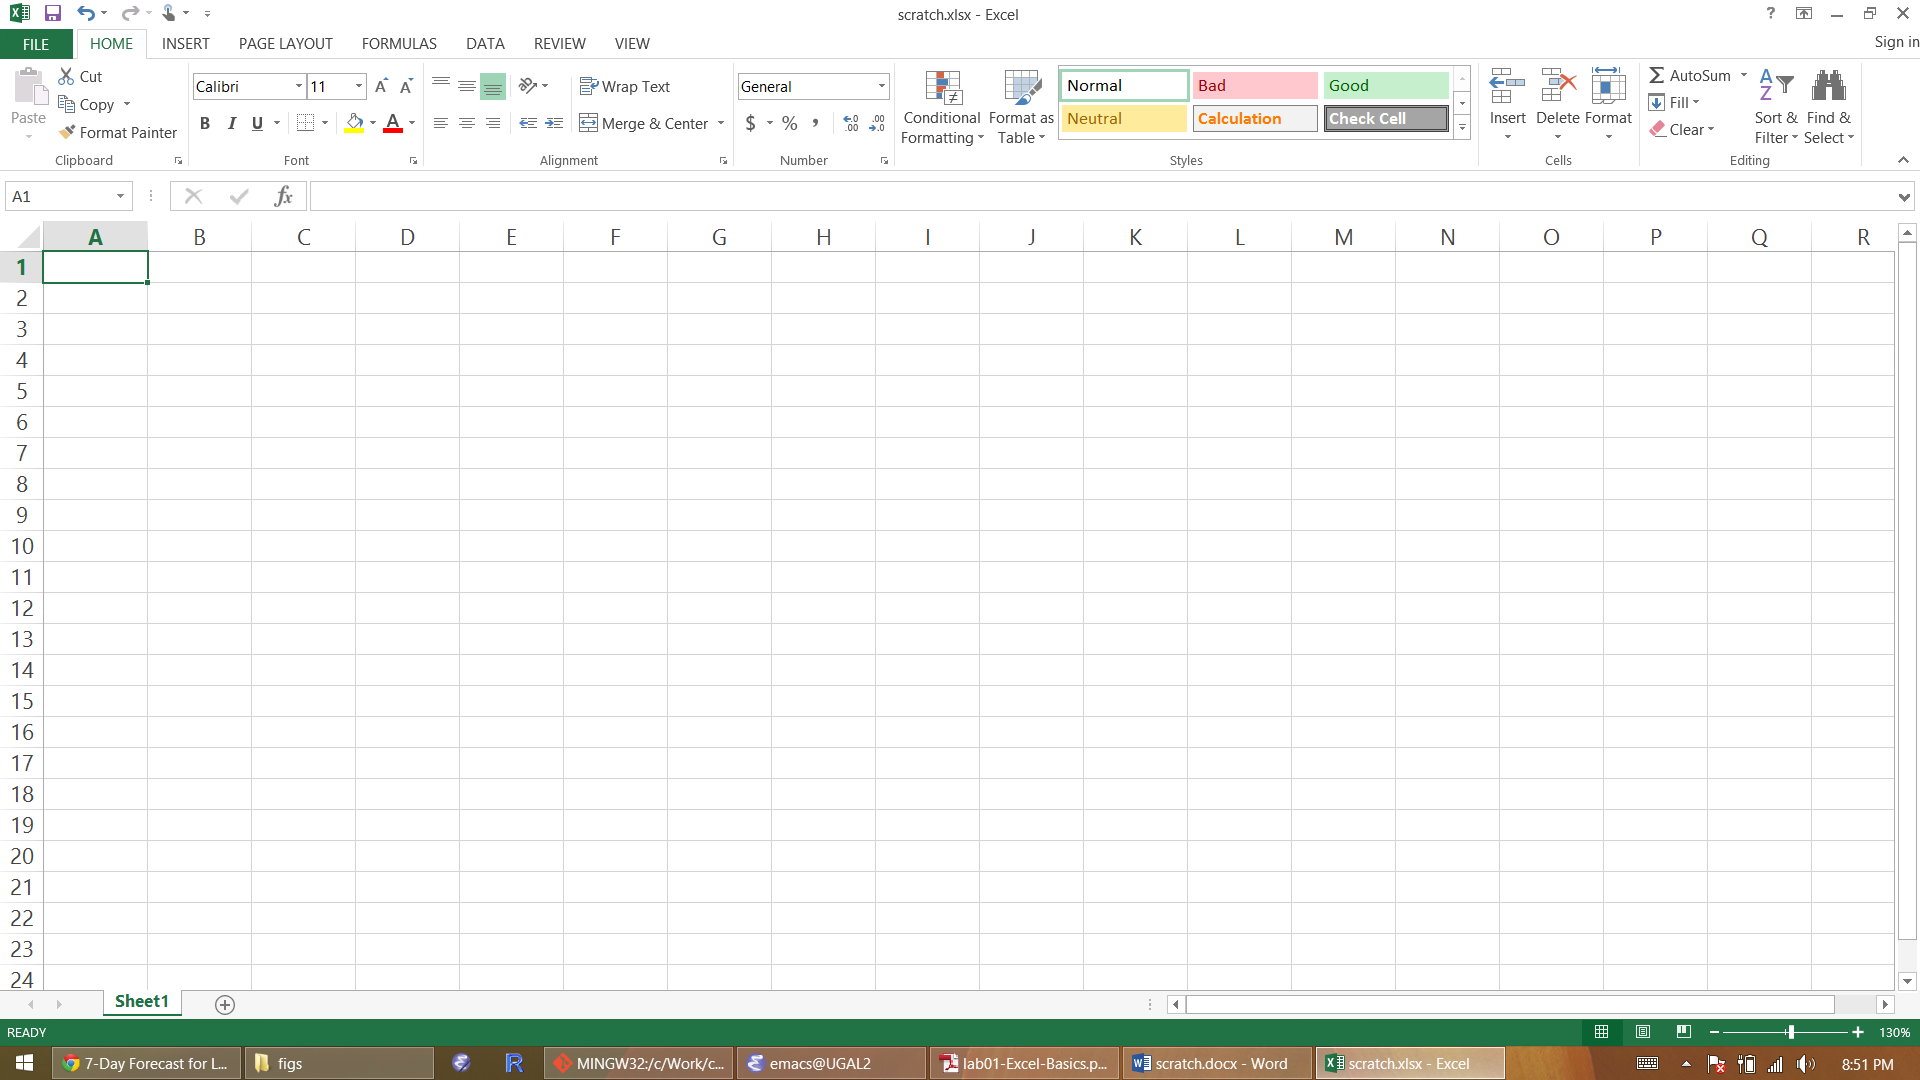
\includegraphics[width=\textwidth]{figs/excel}}
  \end{center}
%  \note{Describe structure... quick access toolbar, ribbon, sheets, workbooks, etc...}
\end{frame}


\section{Referencing}


\begin{frame}
  \frametitle{Column B}
  \fbox{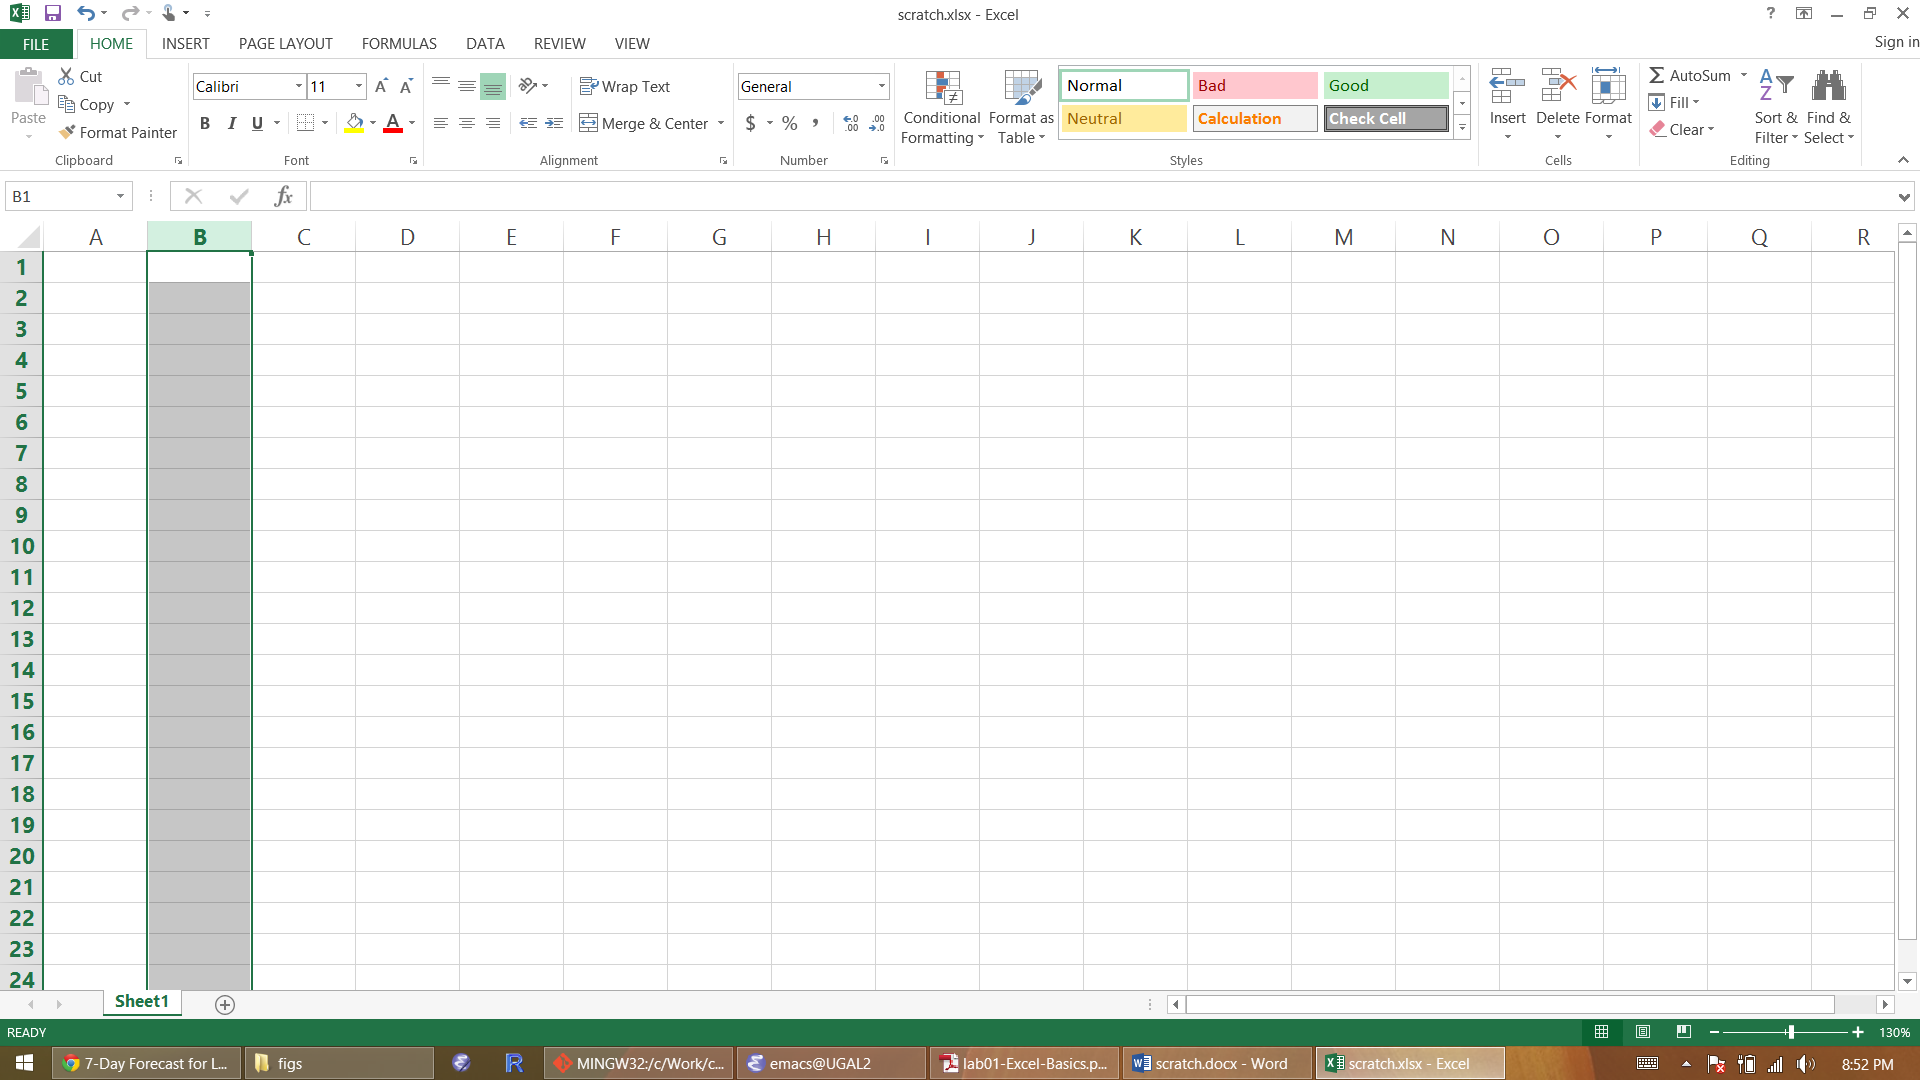
\includegraphics[width=\textwidth]{figs/columnB}}
\end{frame}


\begin{frame}
  \frametitle{Row 3}
  \fbox{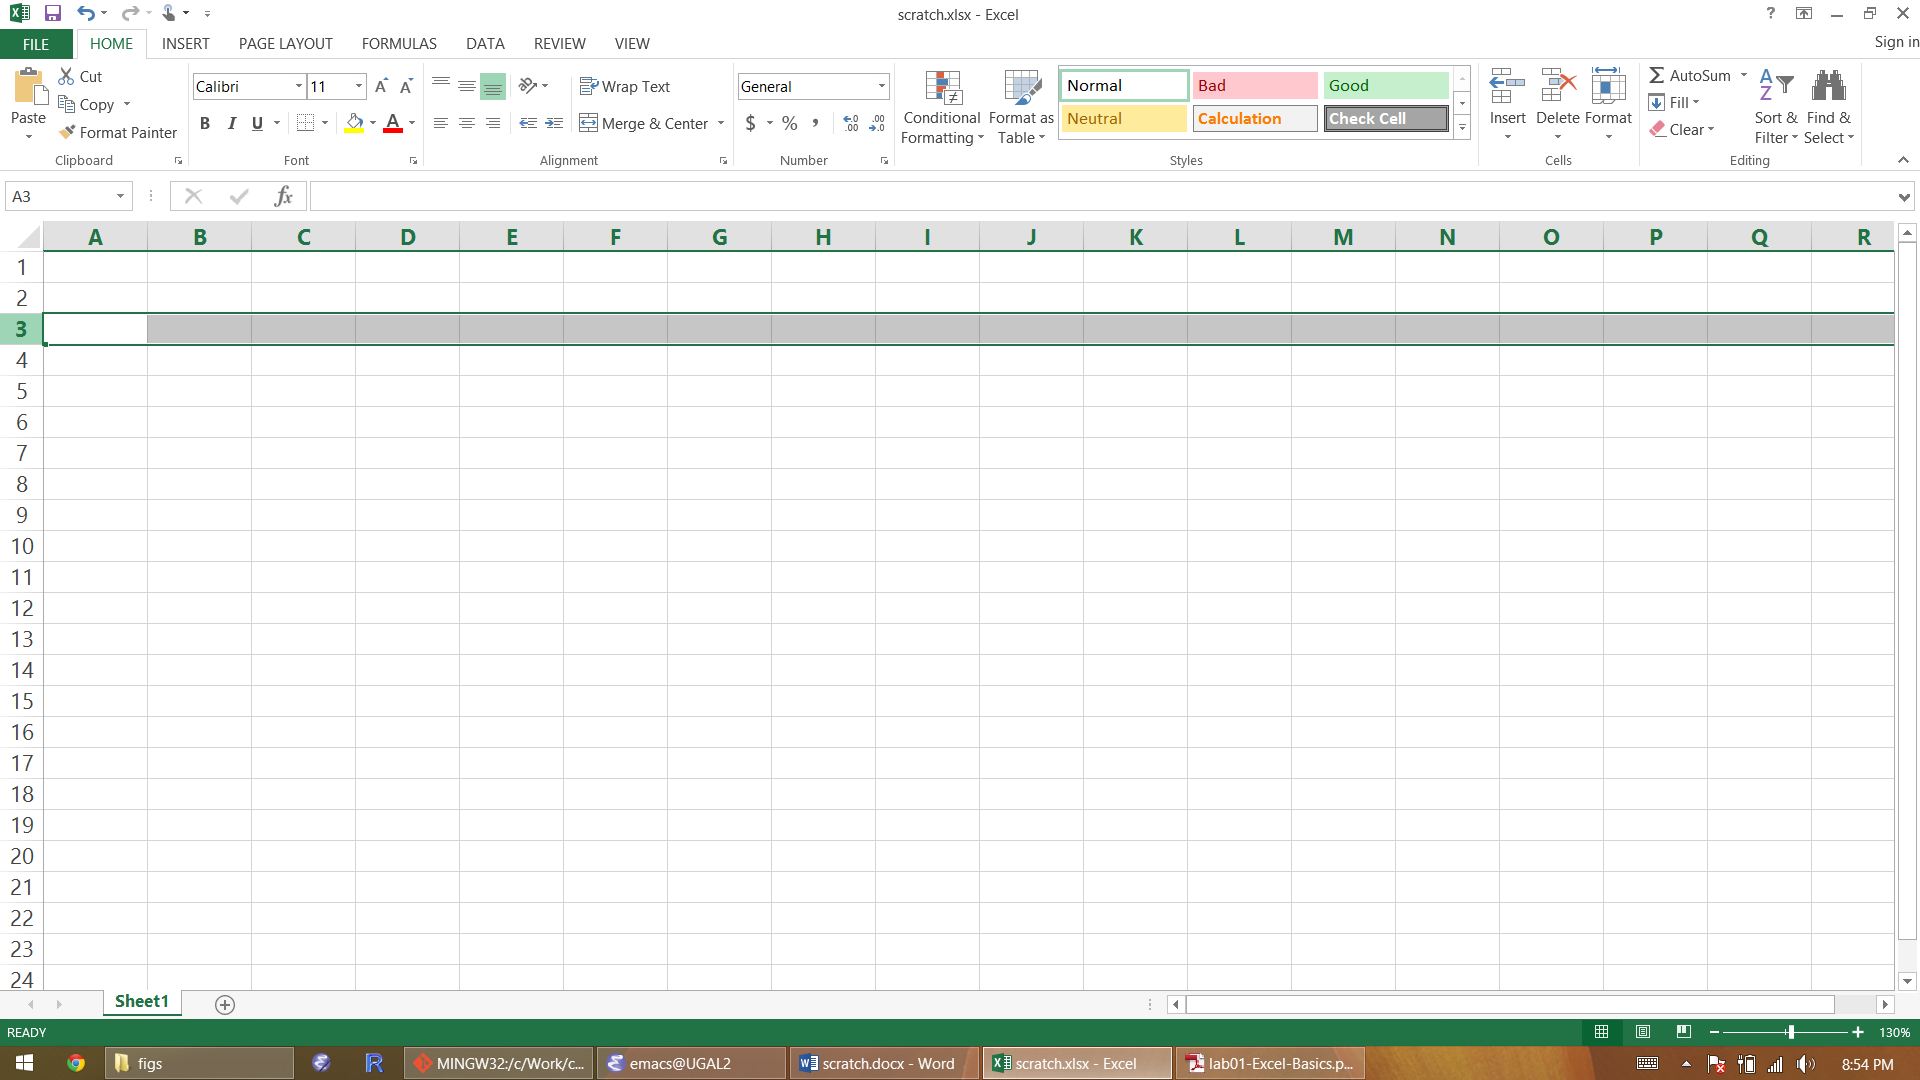
\includegraphics[width=\textwidth]{figs/row3}}
\end{frame}



\begin{frame}
  \frametitle{Cell B3}
  \fbox{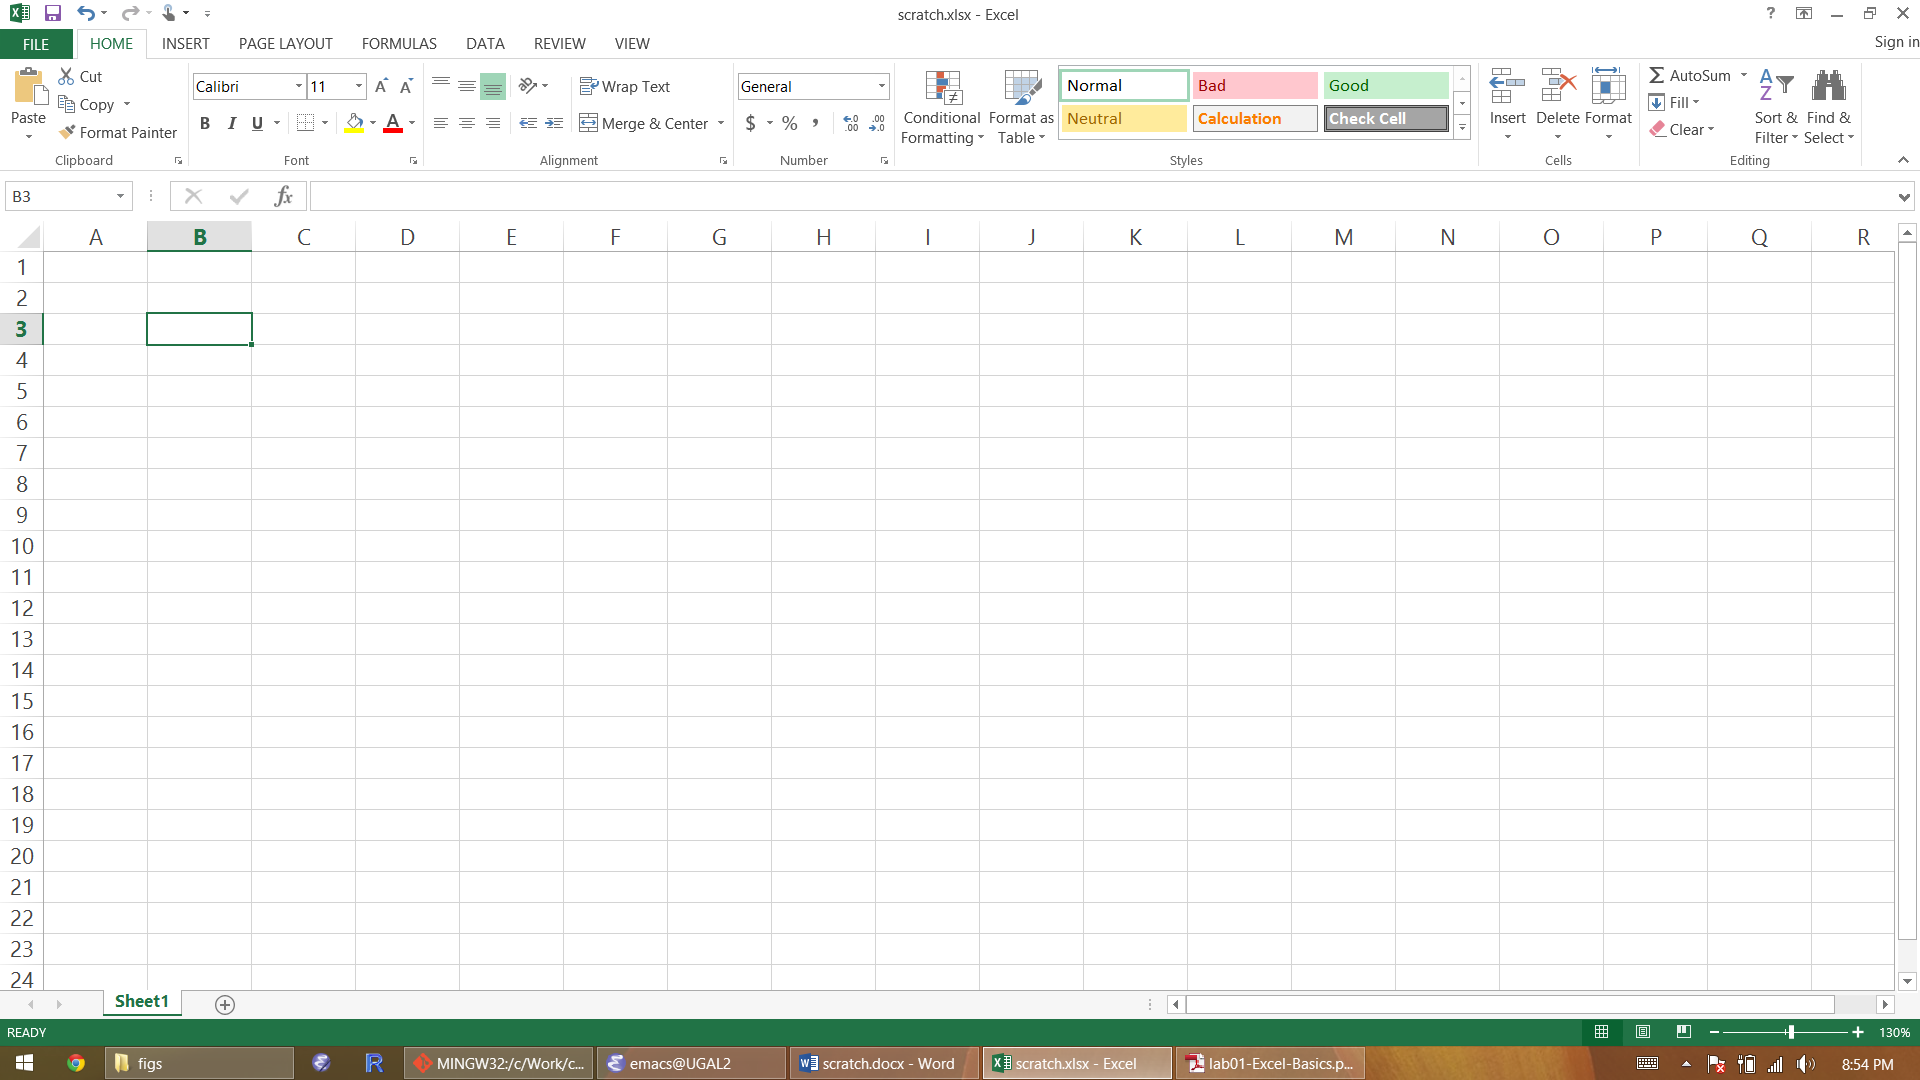
\includegraphics[width=\textwidth]{figs/cellB3}}
\end{frame}



\begin{frame}
  \frametitle{Create Sequence Using Auto-fill}
  \fbox{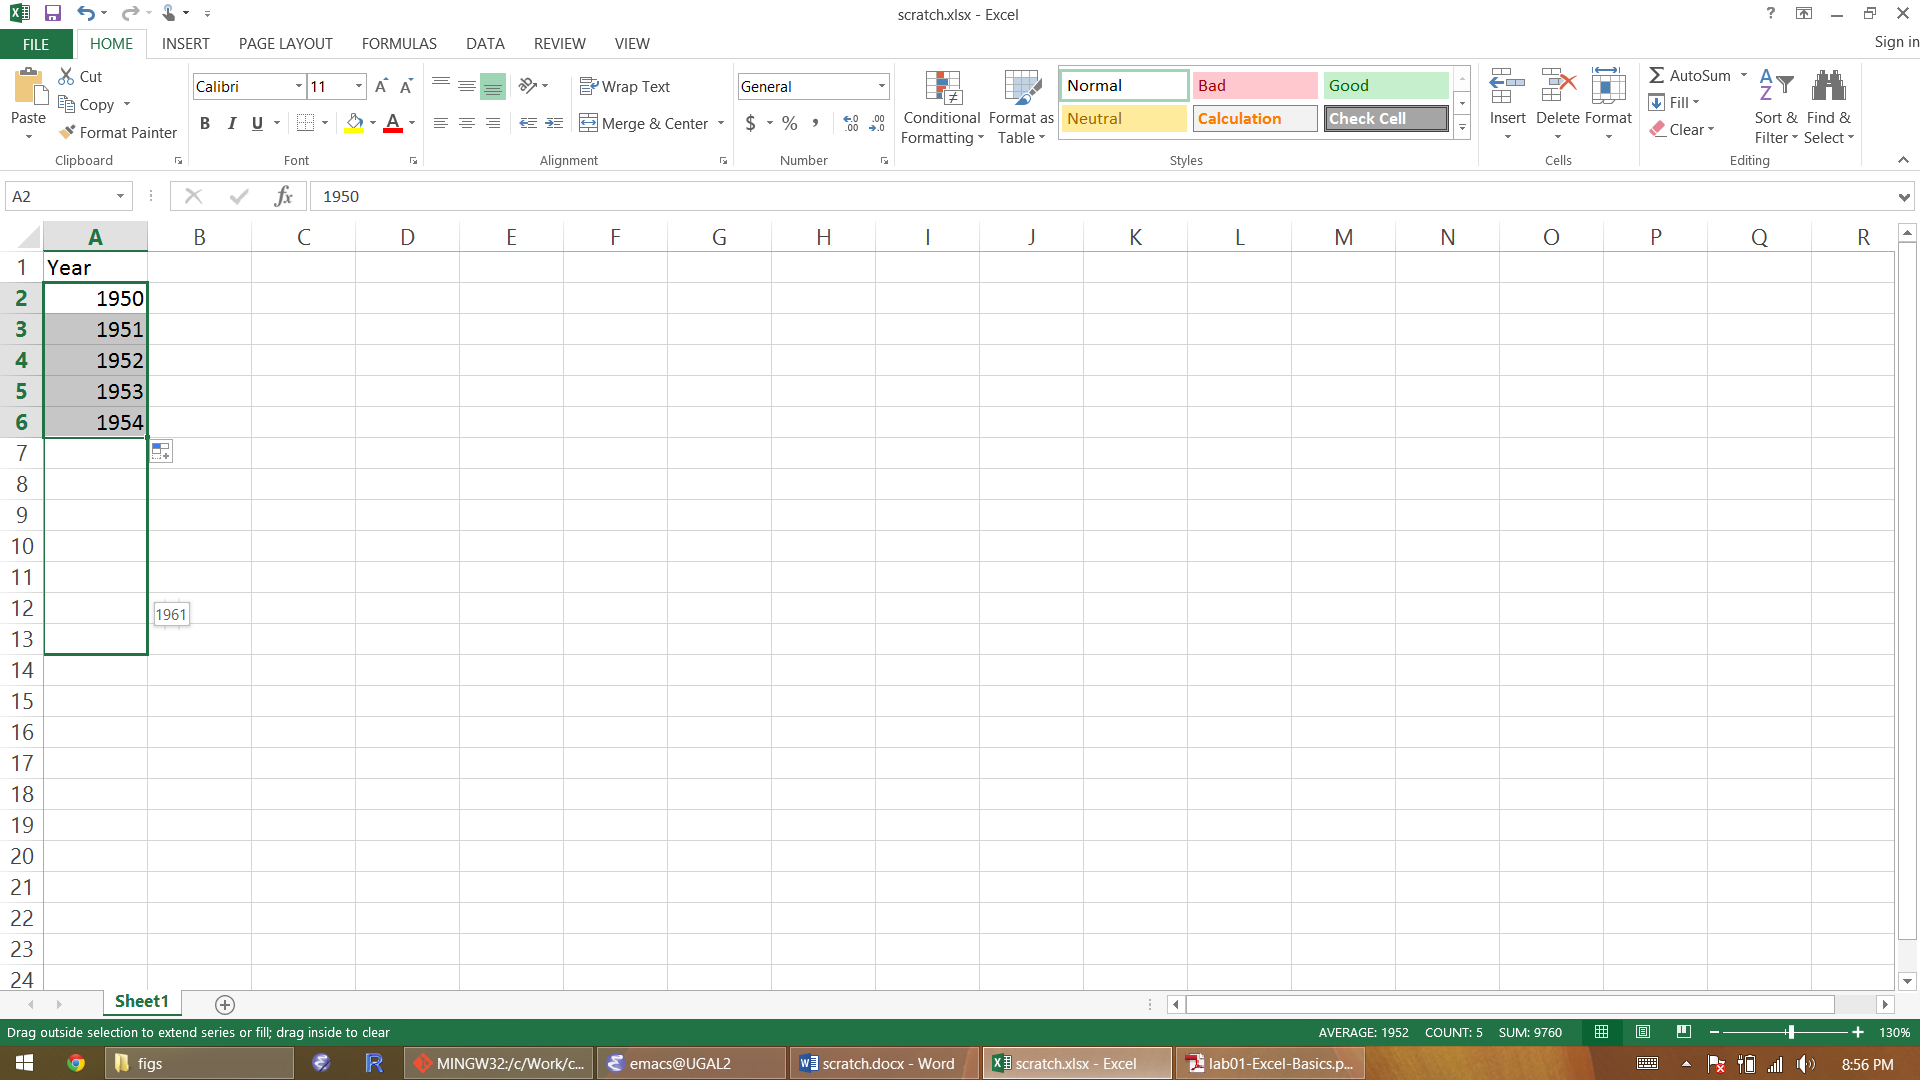
\includegraphics[width=\textwidth]{figs/sequence}}
\end{frame}


\begin{frame}
  \frametitle{Relative Cell References}
  \only<1>{\fbox{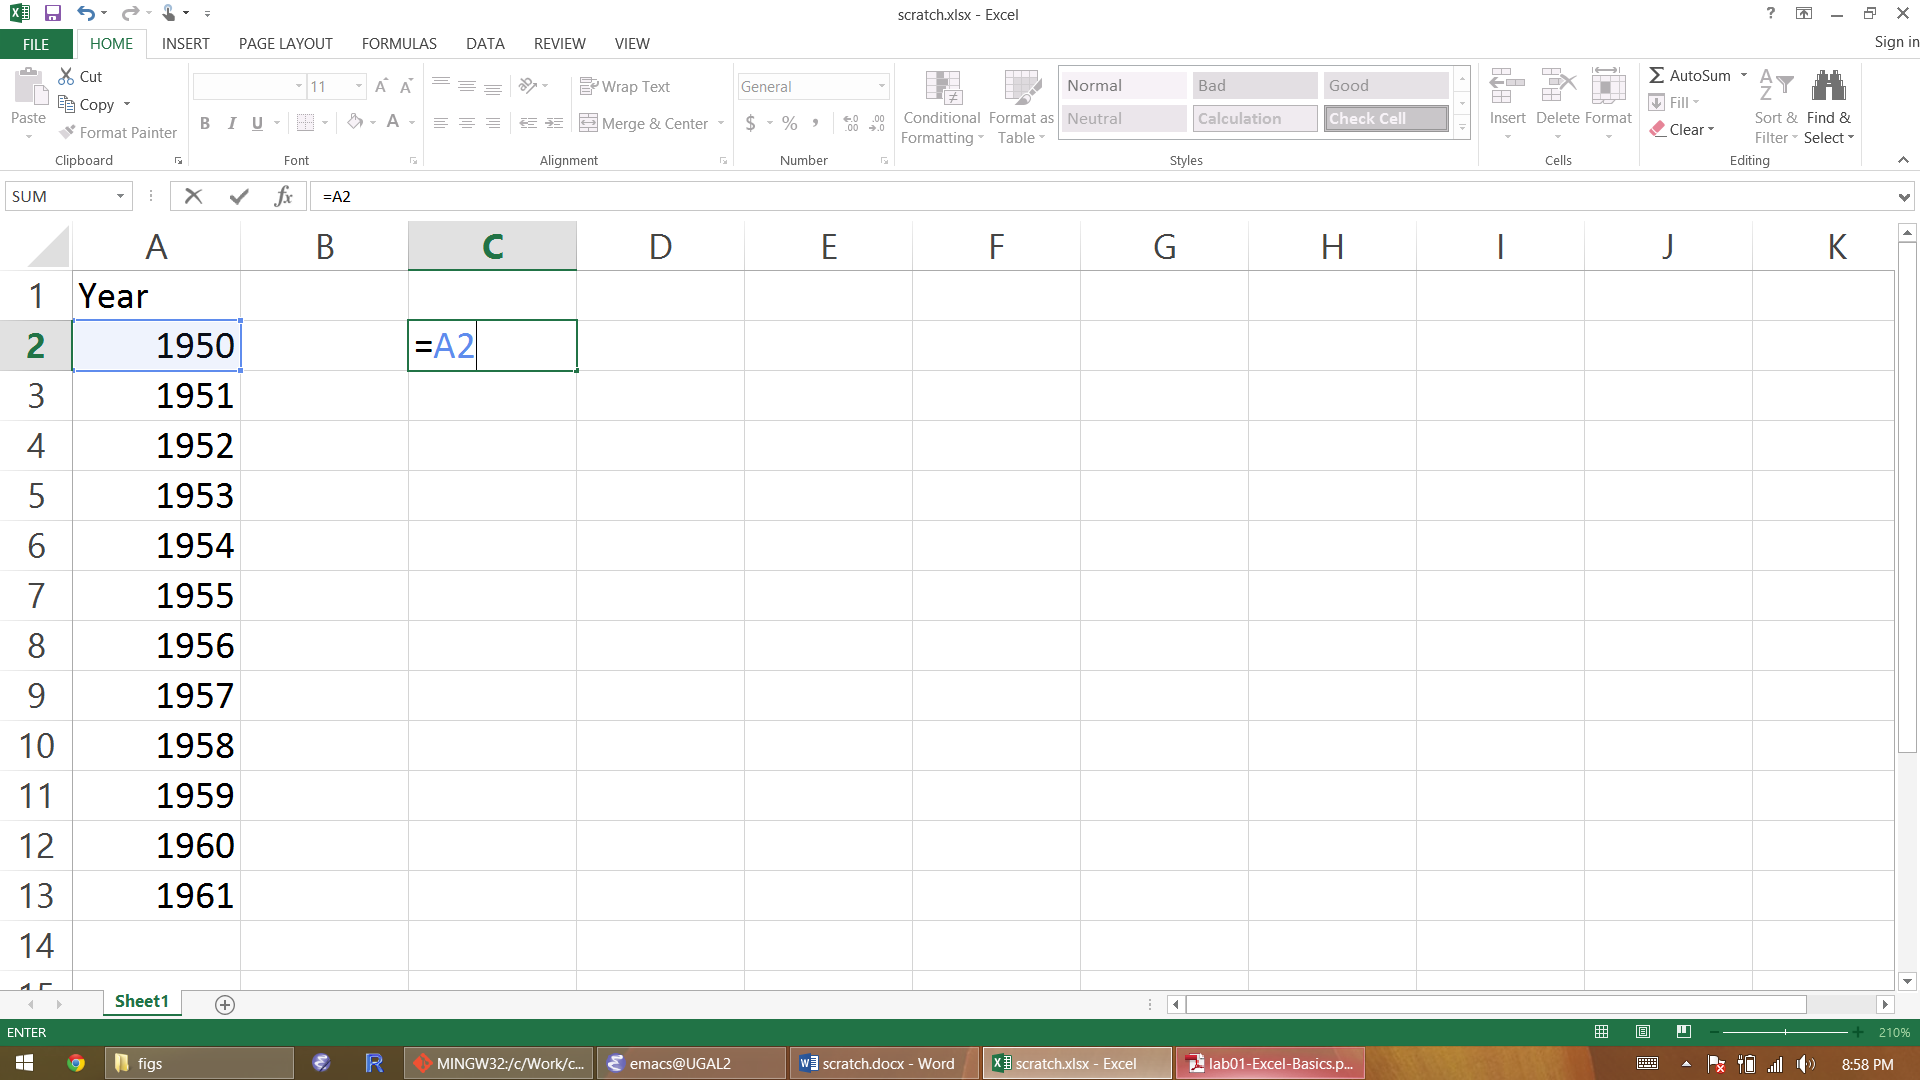
\includegraphics[width=\textwidth]{figs/relative-ref}}}
  \only<2 | handout:0>{\fbox{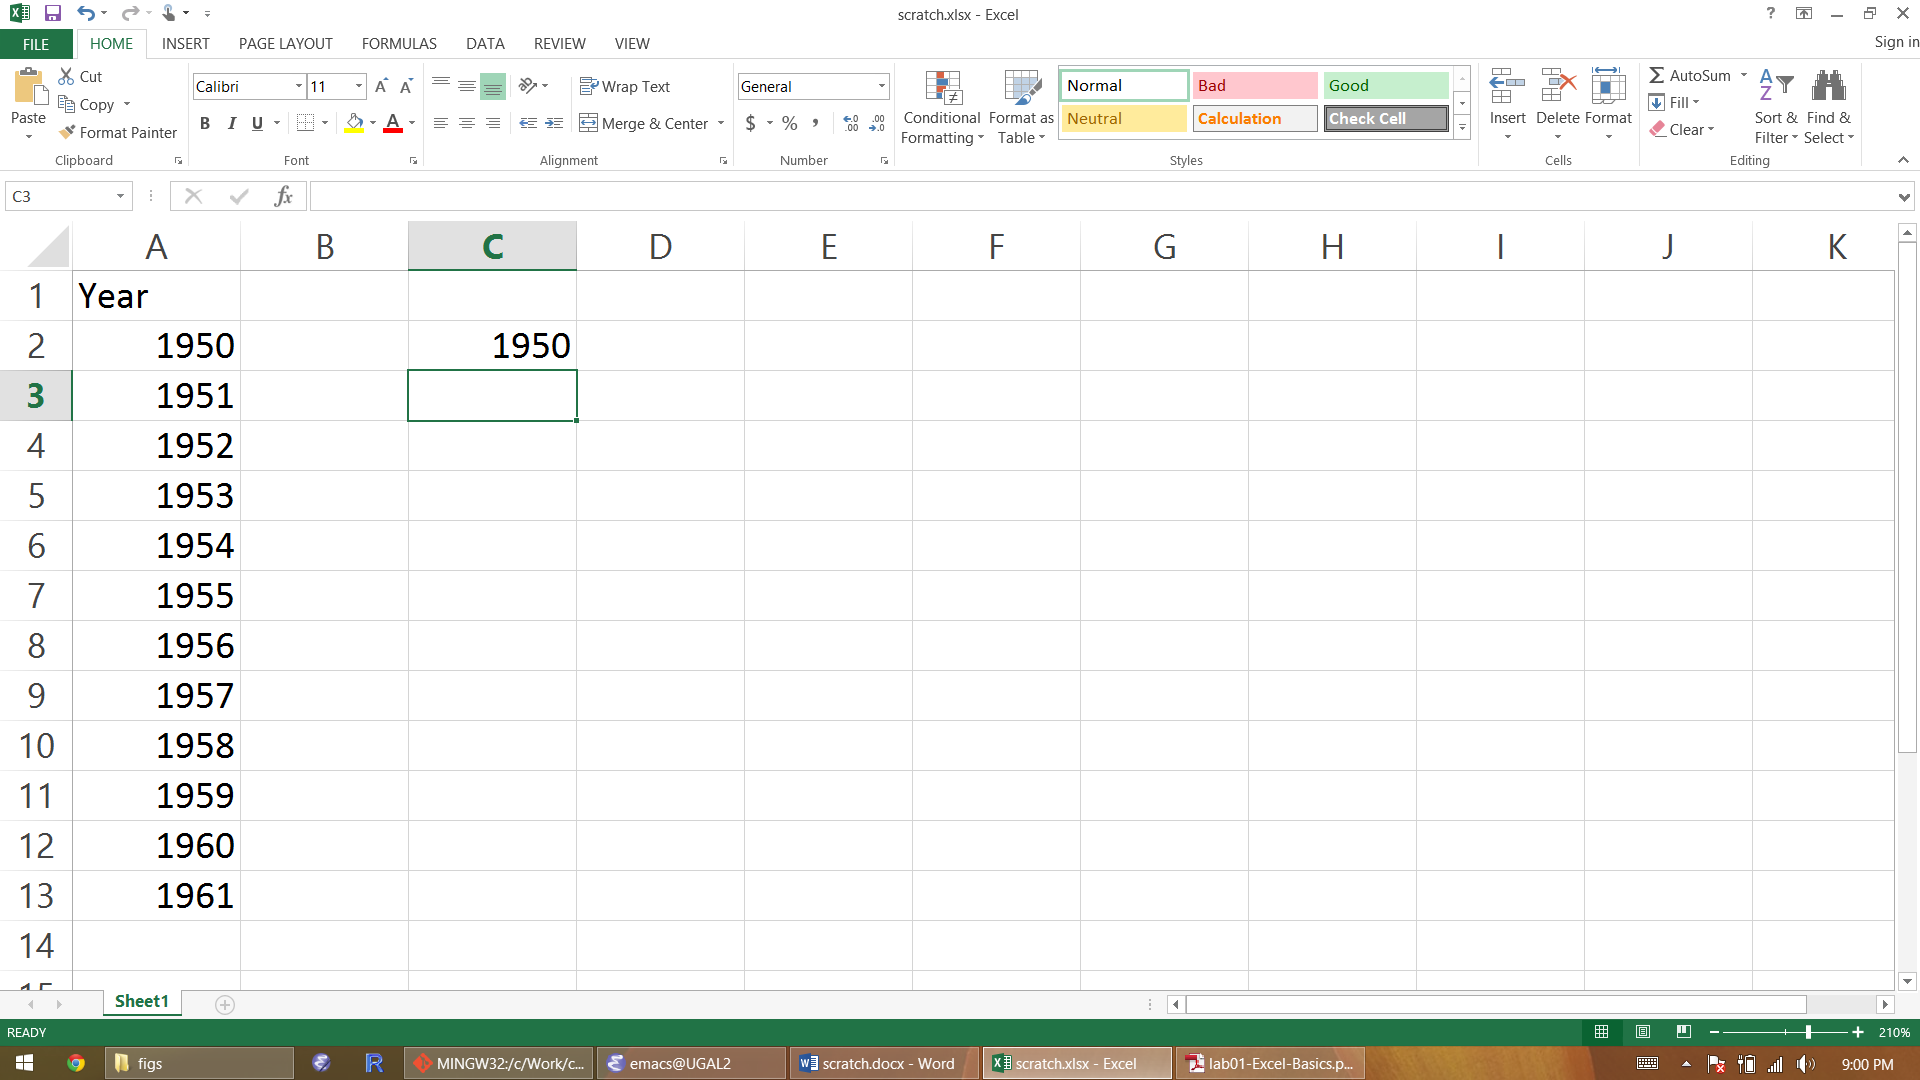
\includegraphics[width=\textwidth]{figs/relative-ref2}}}
  \begin{center}
    Cell C2 will take on the value of A2 \\
  \end{center}
\end{frame}


\begin{frame}
  \frametitle{Relative Cell References}
  \fbox{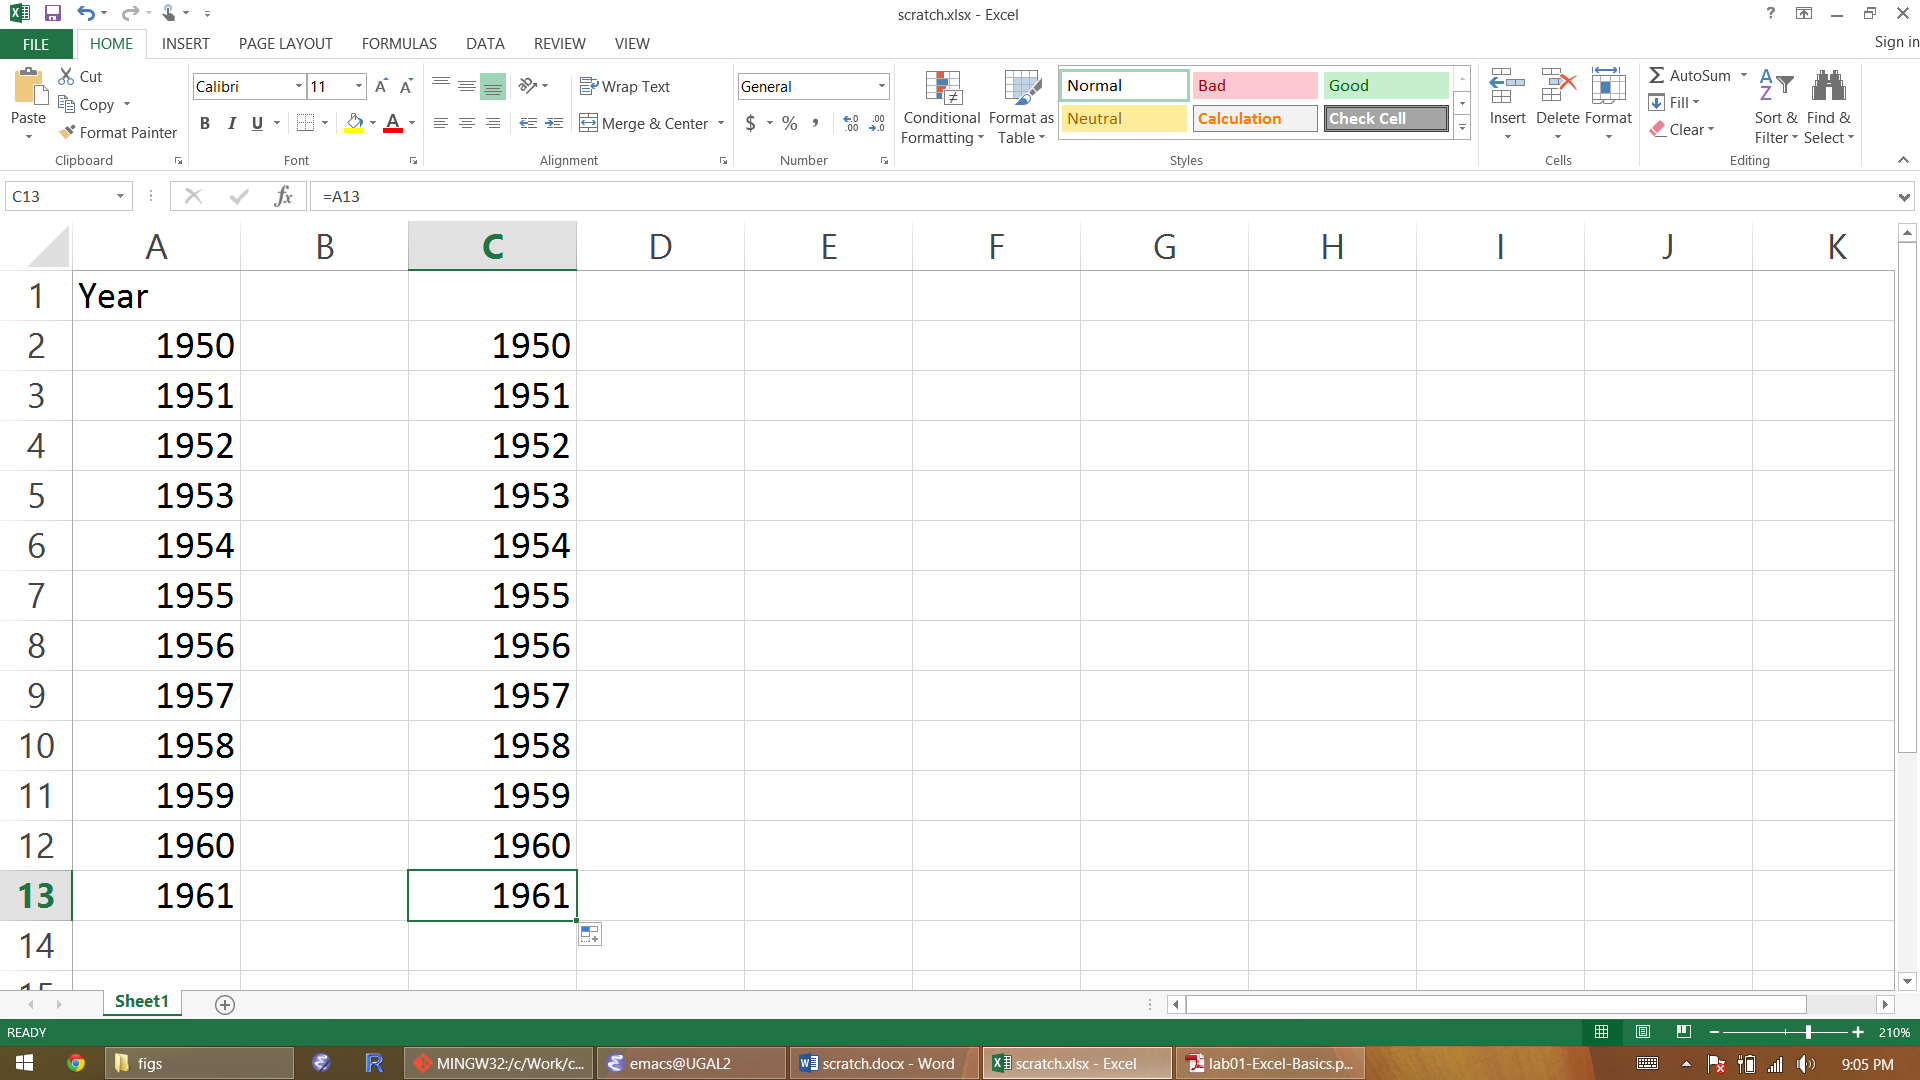
\includegraphics[width=\textwidth]{figs/relative-ref3}}
  \begin{center}
    Values of reference will change when using auto-fill
  \end{center}
\end{frame}


\begin{frame}
  \frametitle{Absolute Cell References}
  \only<1>{\fbox{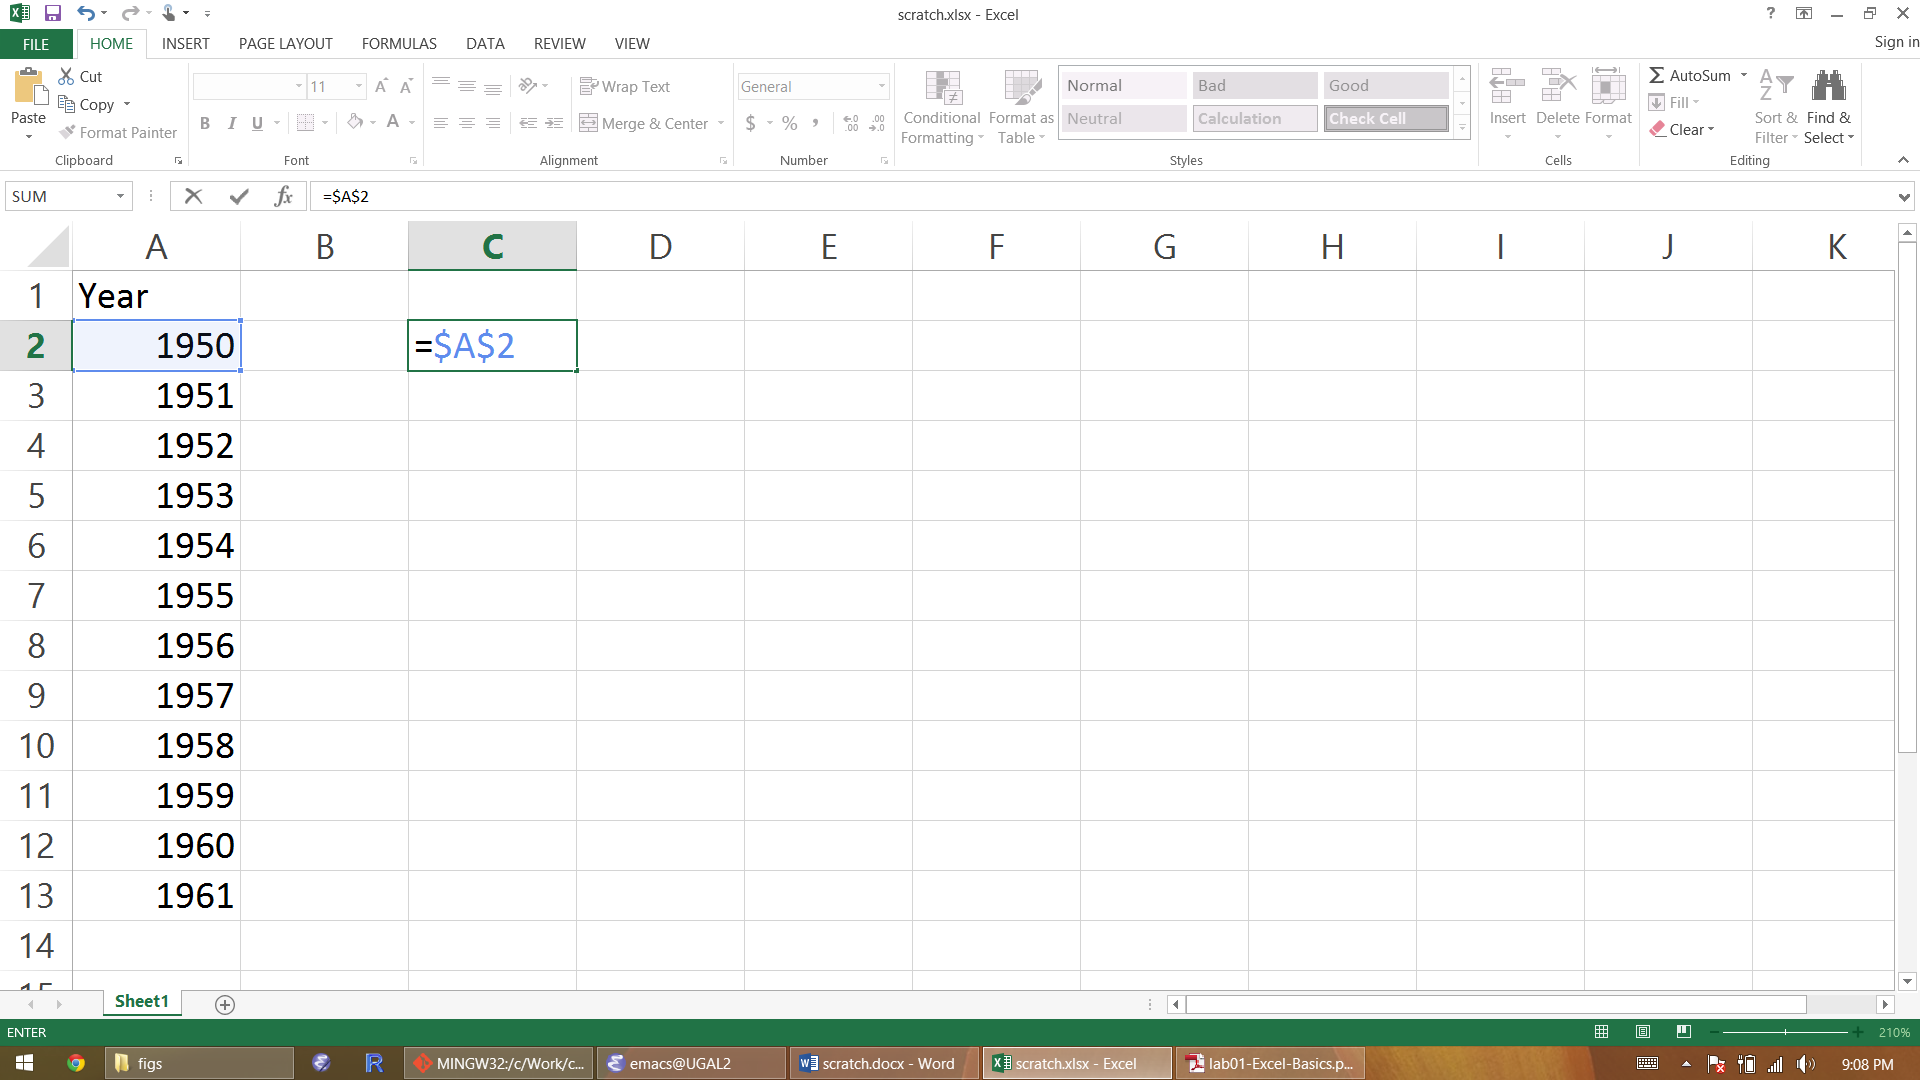
\includegraphics[width=\textwidth]{figs/absolute-ref}}}
  \only<2 | handout:0>{\fbox{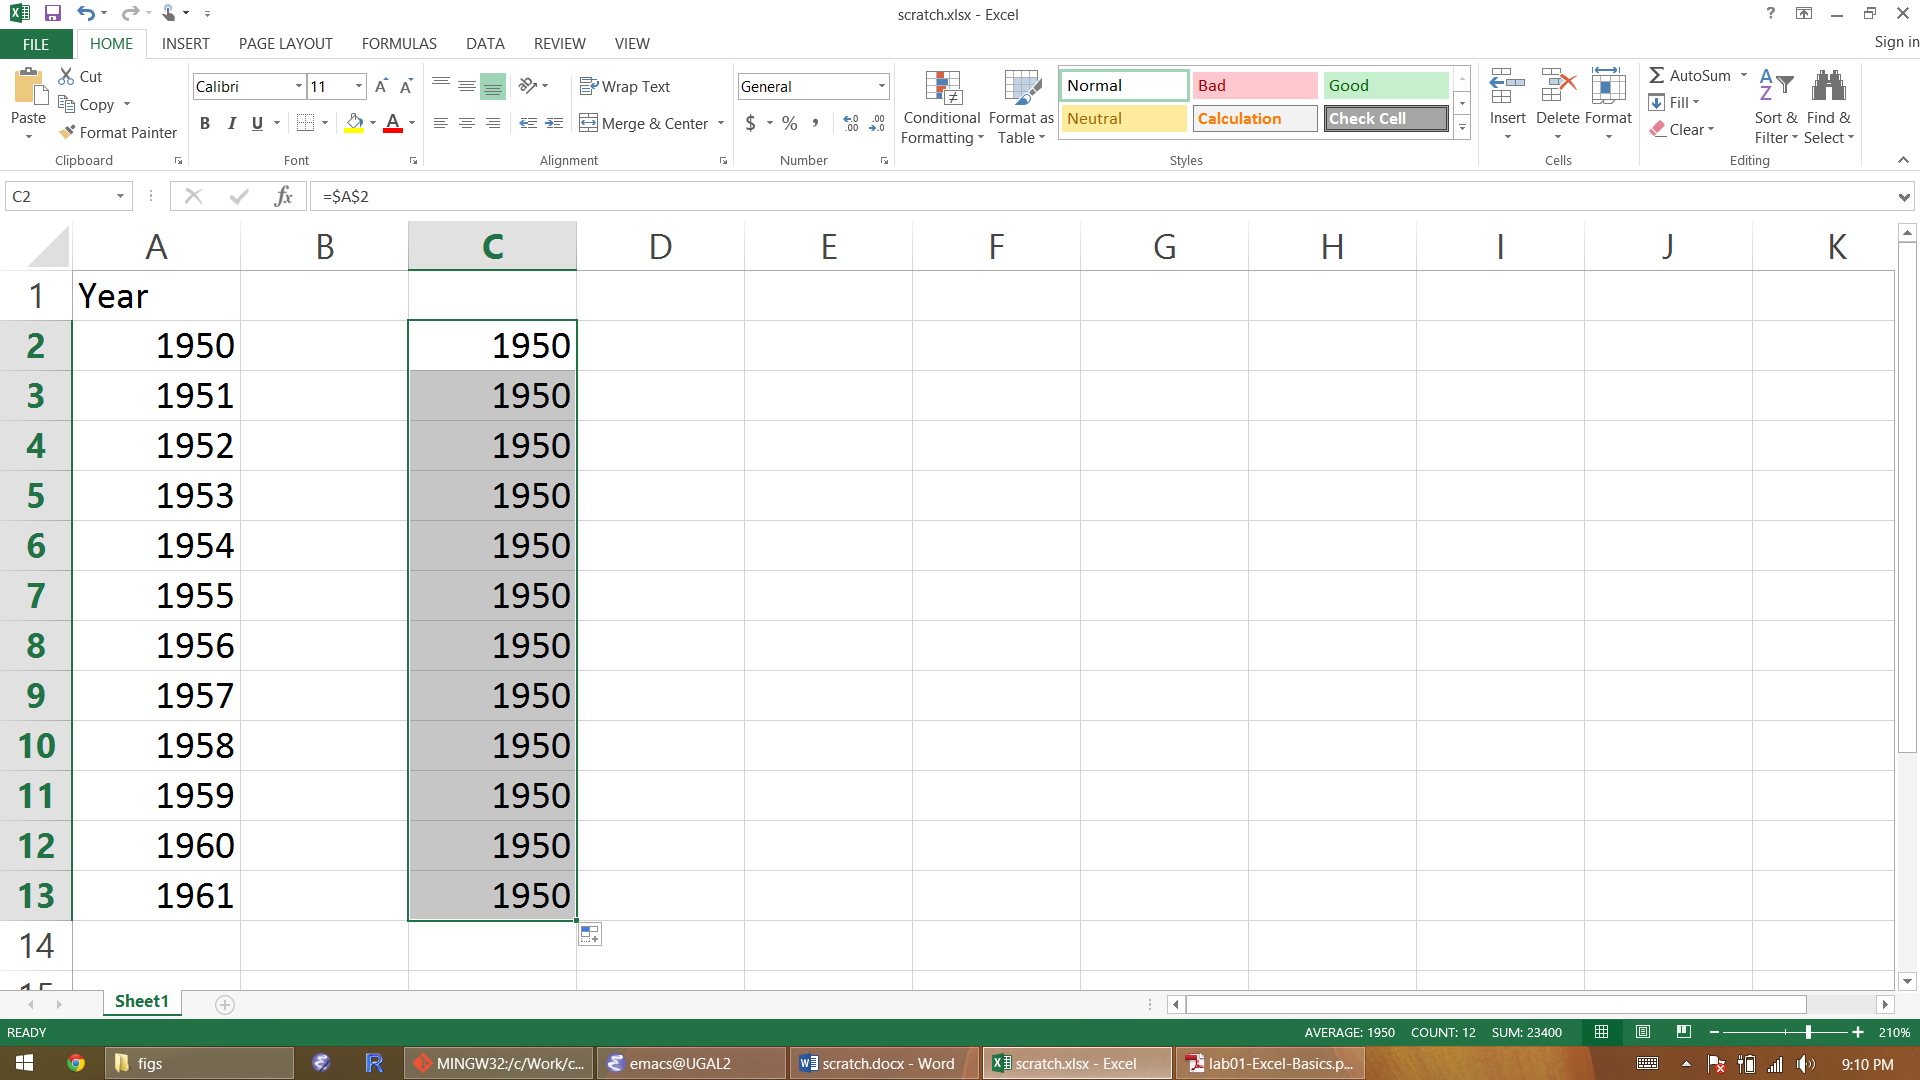
\includegraphics[width=\textwidth]{figs/absolute-ref2}}}
  \begin{center}
    Dollar sign ``locks'' value so that auto-fill won't change it
  \end{center}
\end{frame}


\begin{frame}
  \frametitle{Partial Cell References}
  \fbox{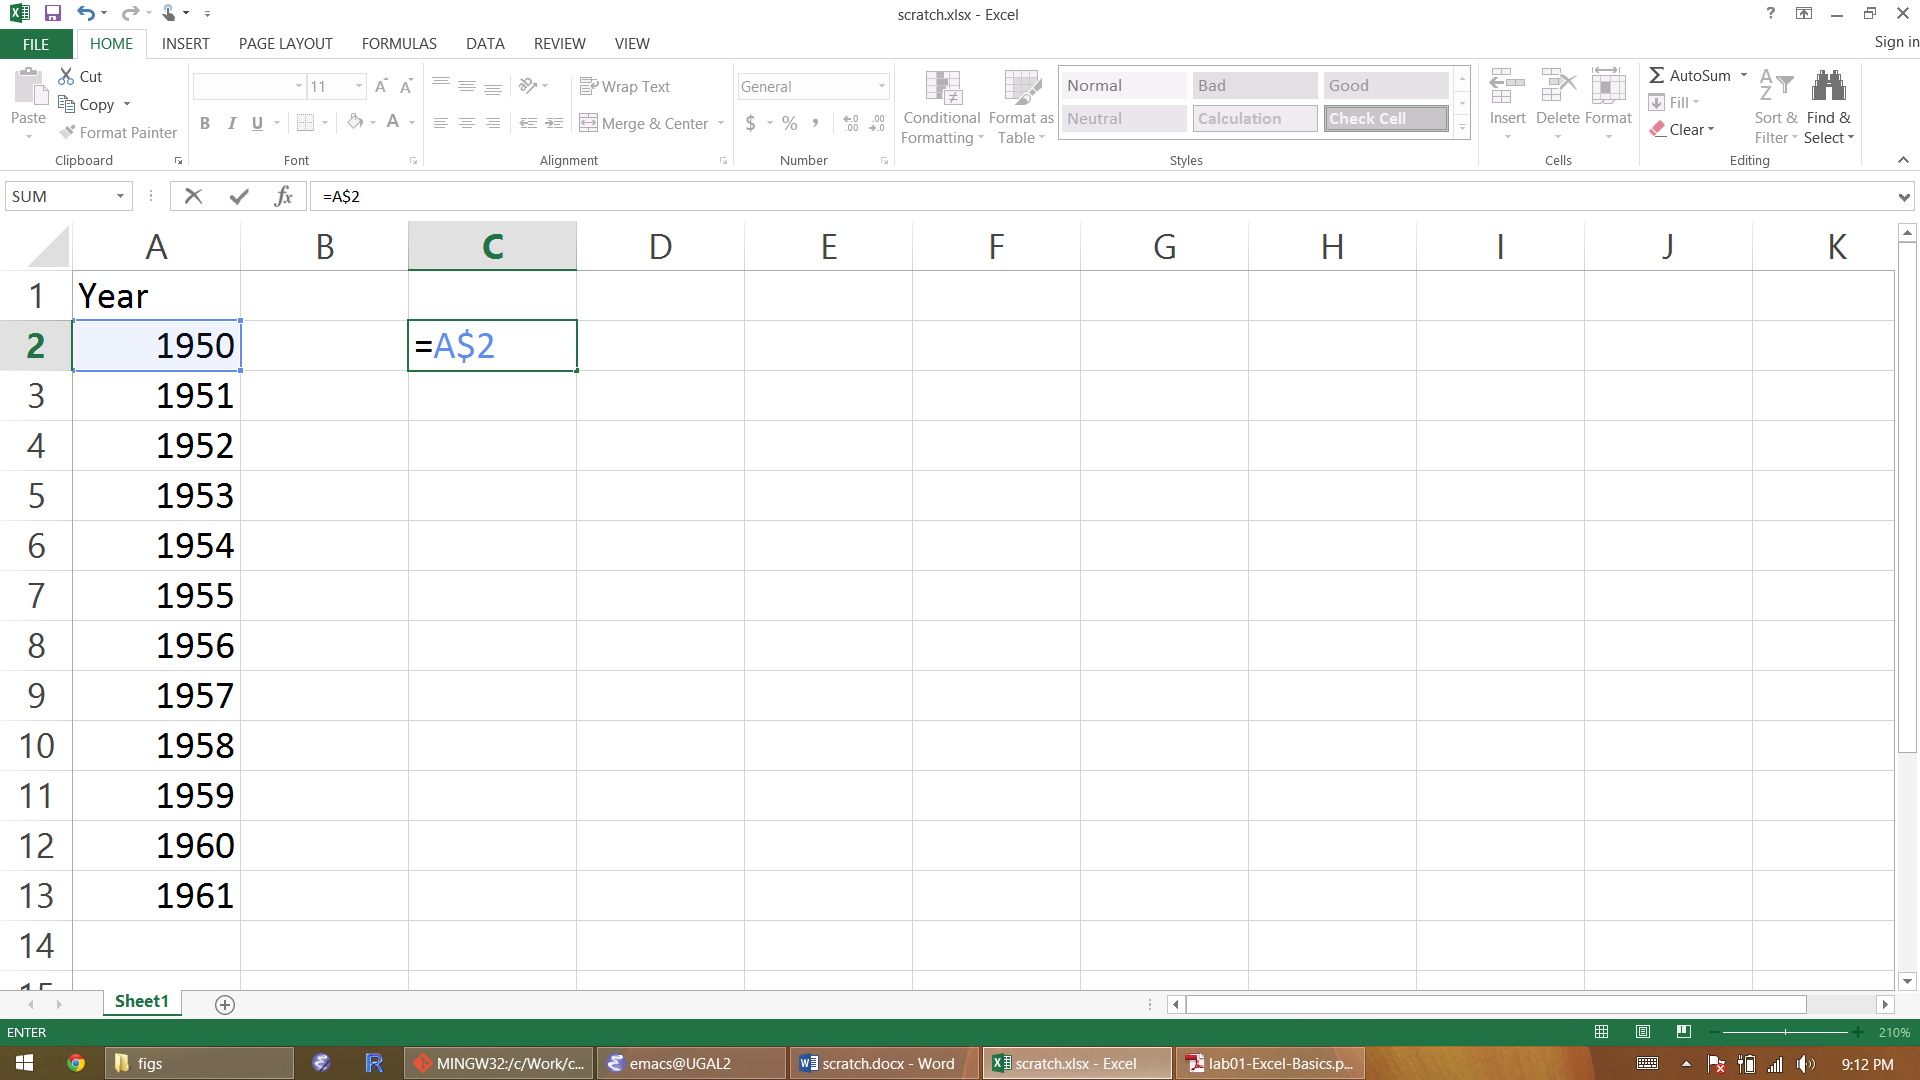
\includegraphics[width=\textwidth]{figs/partial-ref}}
\end{frame}


\section{Equations}



\begin{frame}
  \frametitle{Equations}
%  \begin{ce}
    \only<1>{\fbox{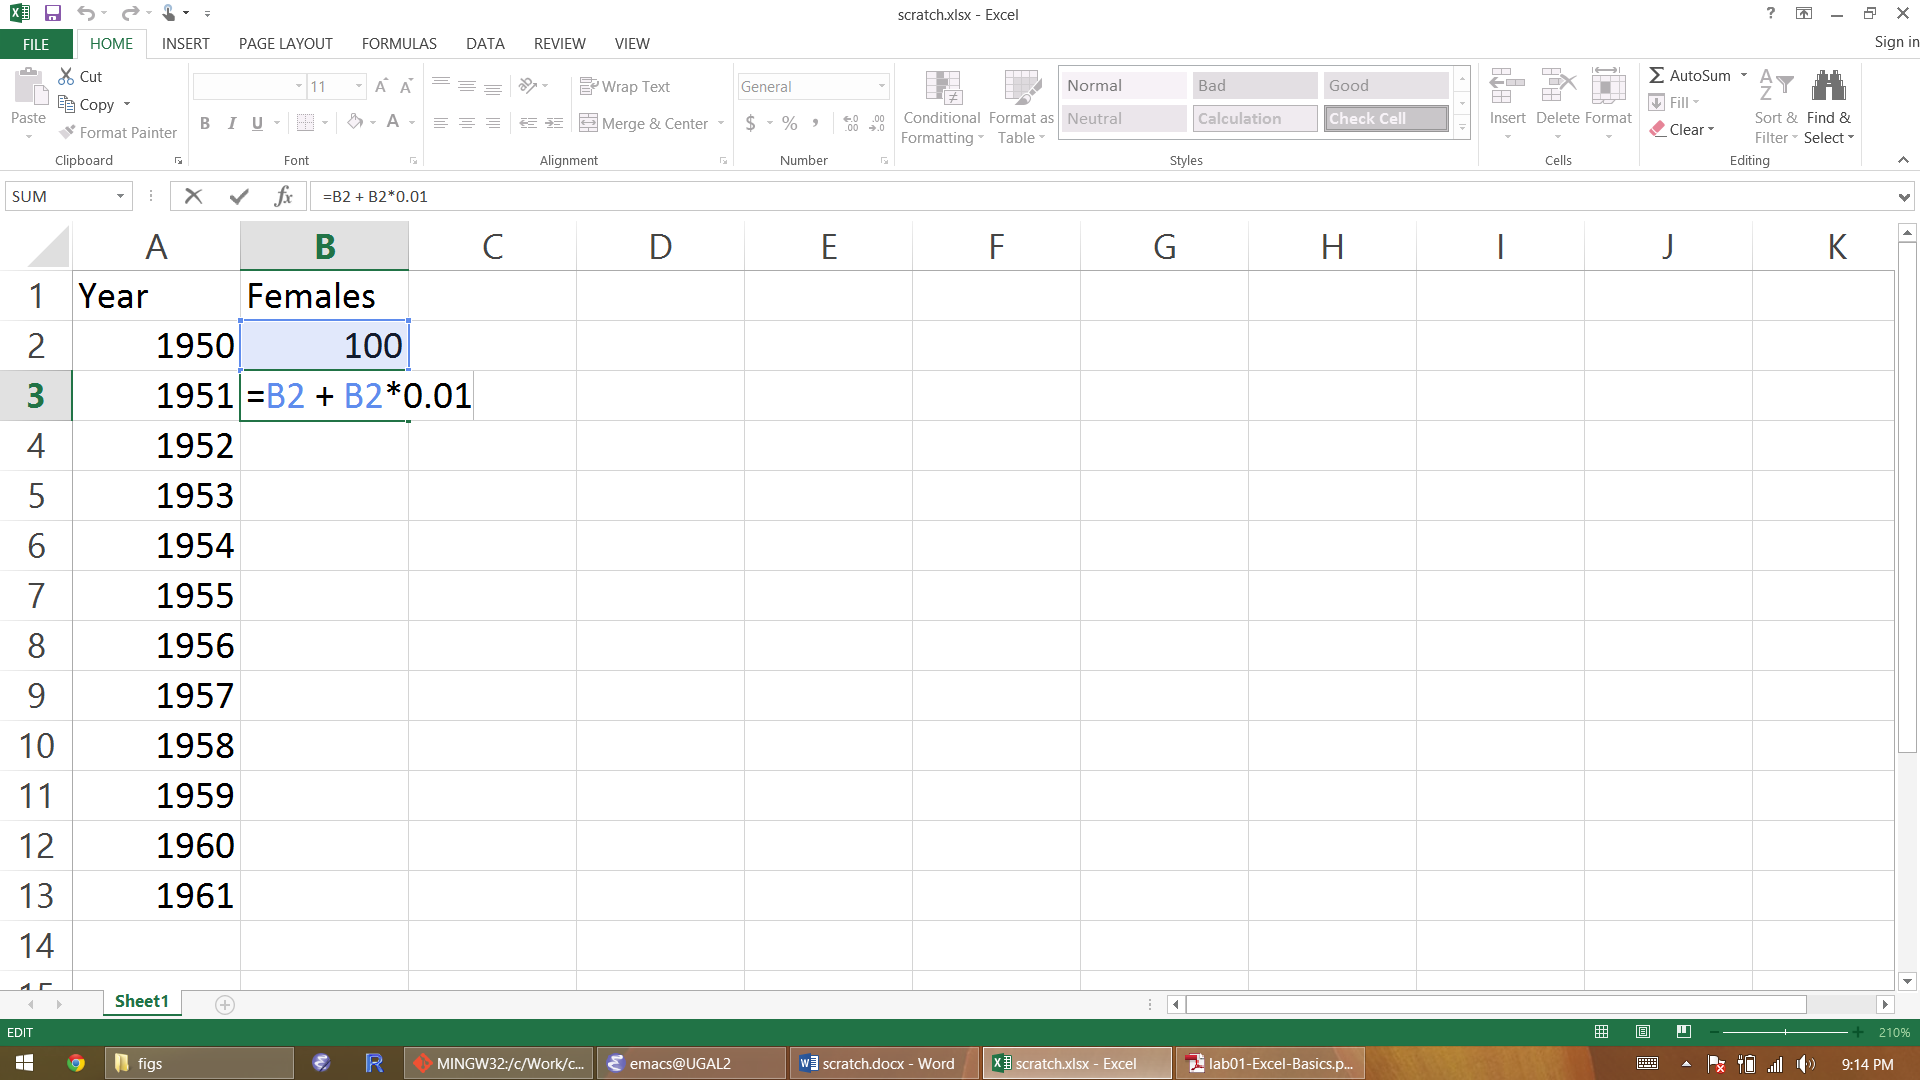
\includegraphics[width=\textwidth]{figs/equation}}}
    \only<2 | handout:0>{\fbox{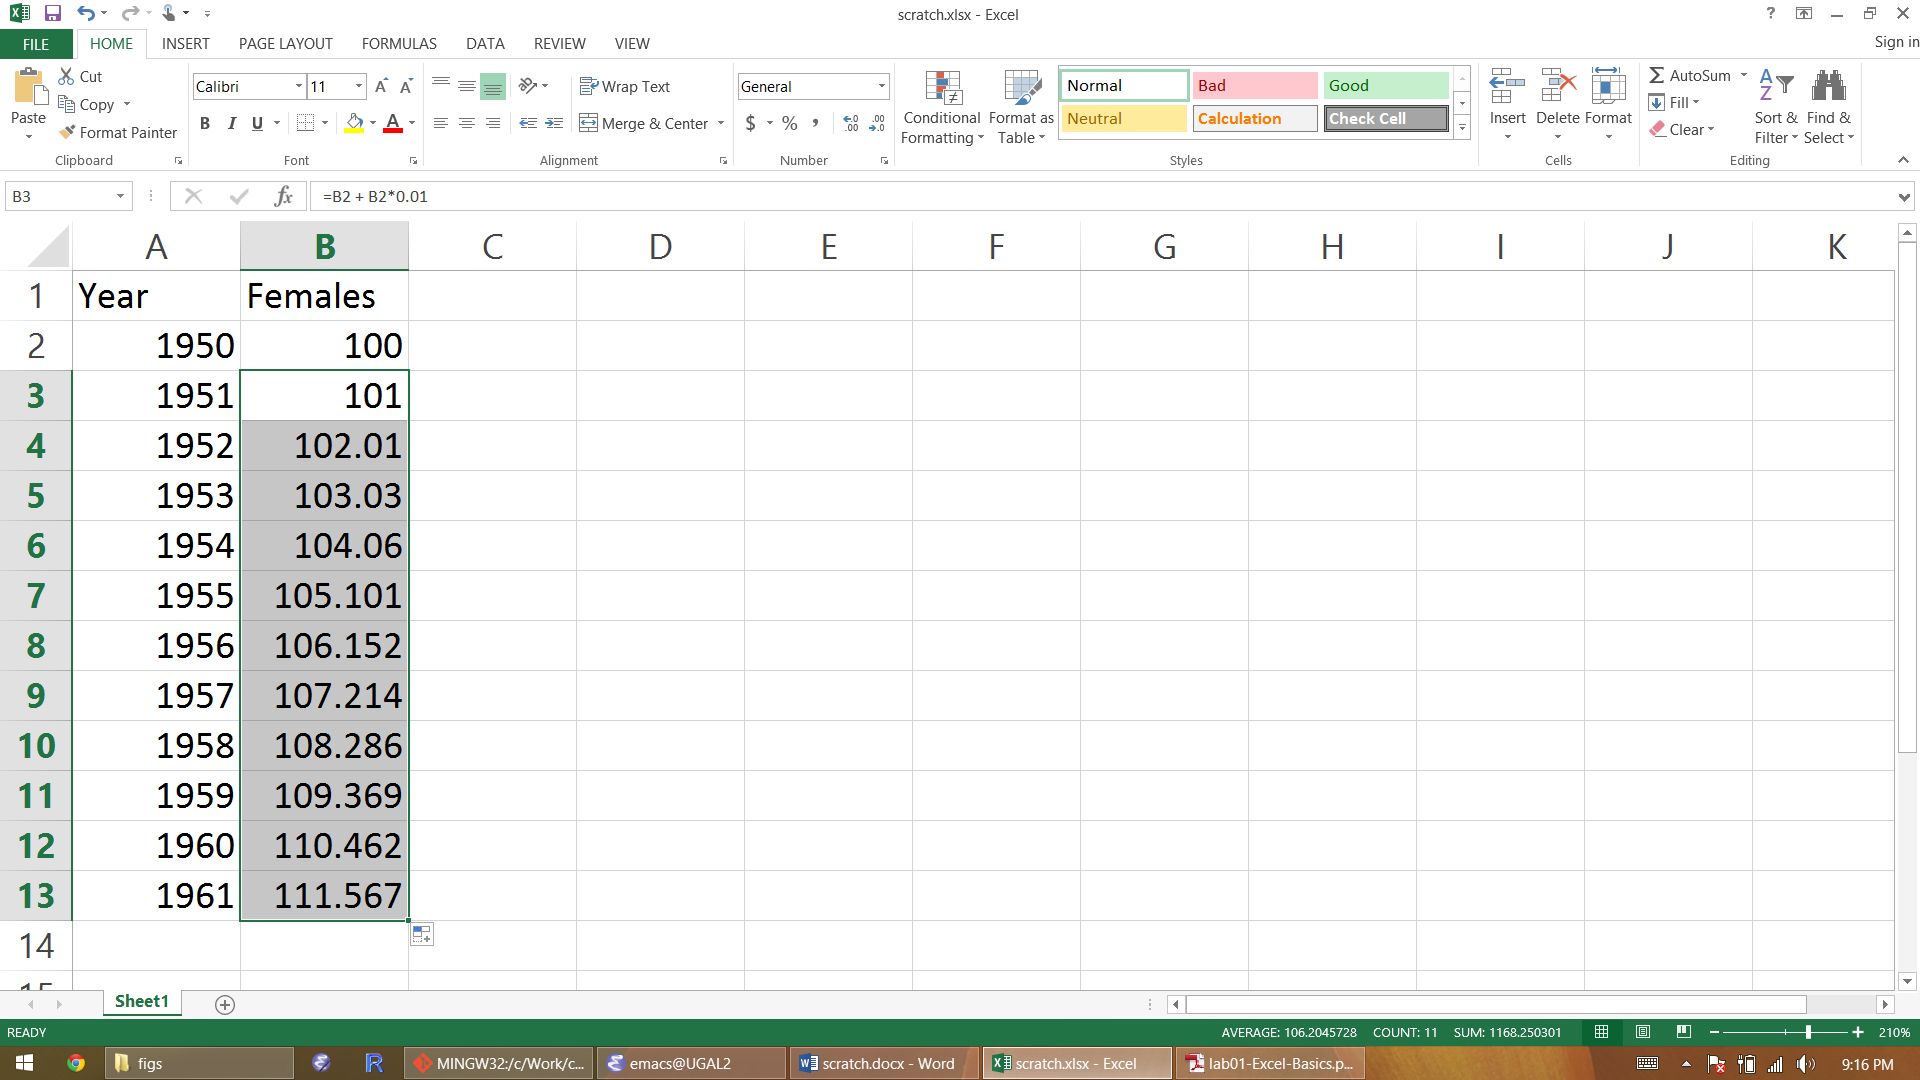
\includegraphics[width=\textwidth]{figs/equation2}}}
%  \end{overprint}
\end{frame}



\begin{frame}
  \frametitle{Equations}
    \only<1>{\fbox{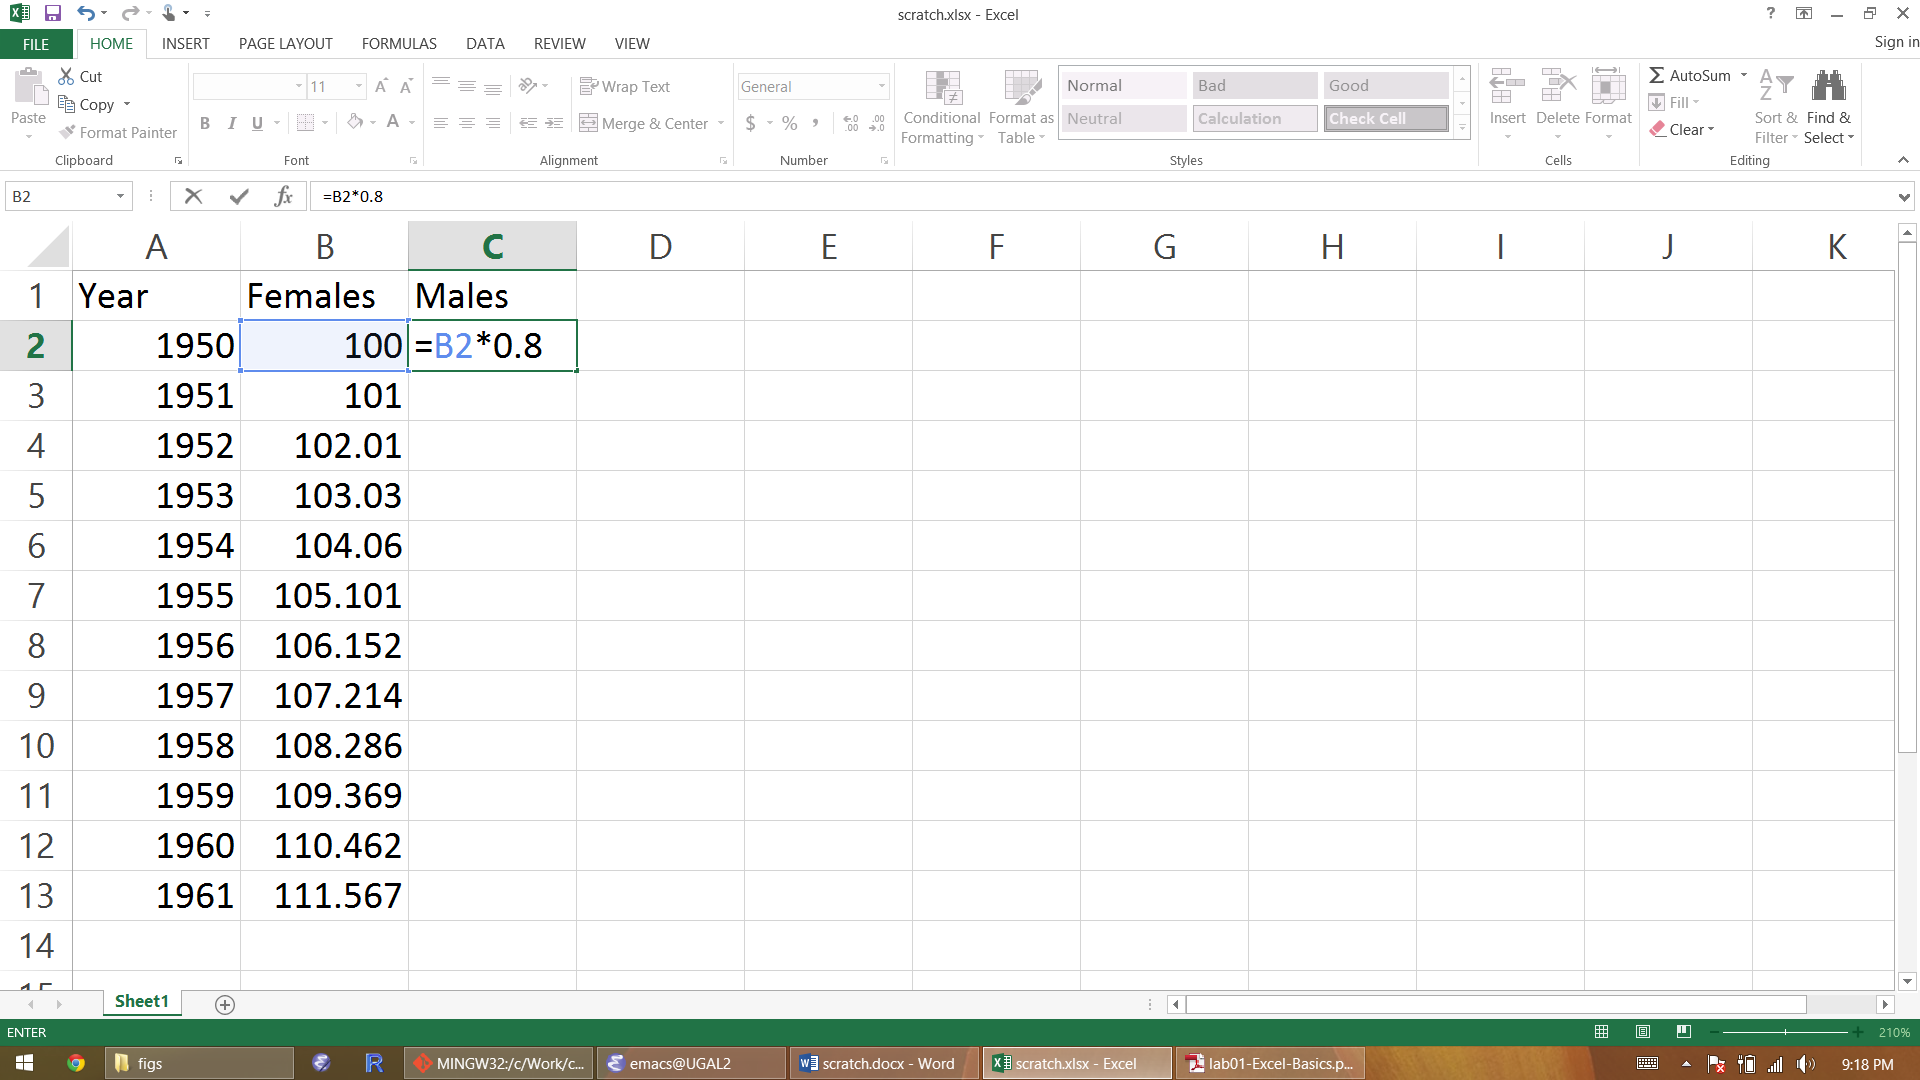
\includegraphics[width=\textwidth]{figs/equation3}}}
    \only<2 | handout:0>{\fbox{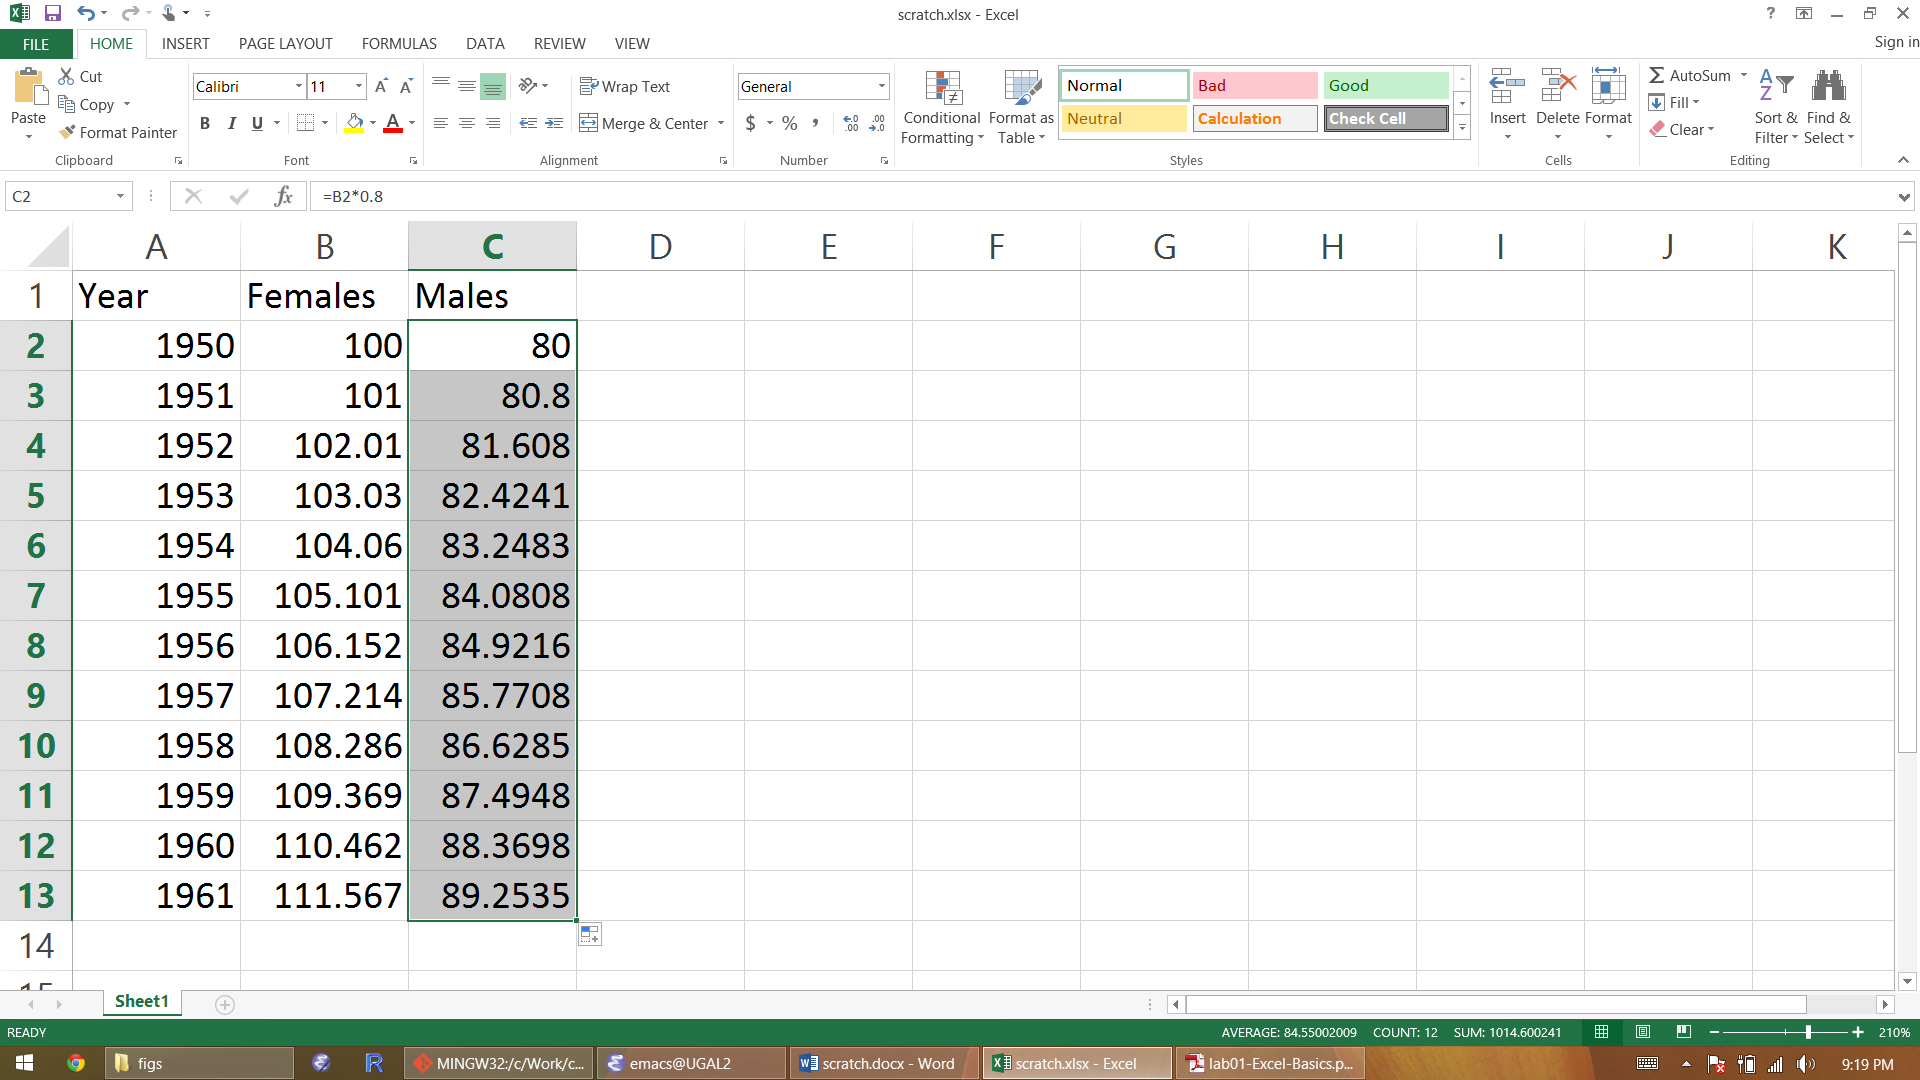
\includegraphics[width=\textwidth]{figs/equation4}}}
\end{frame}



\begin{frame}
  \frametitle{Formulas}
  \fbox{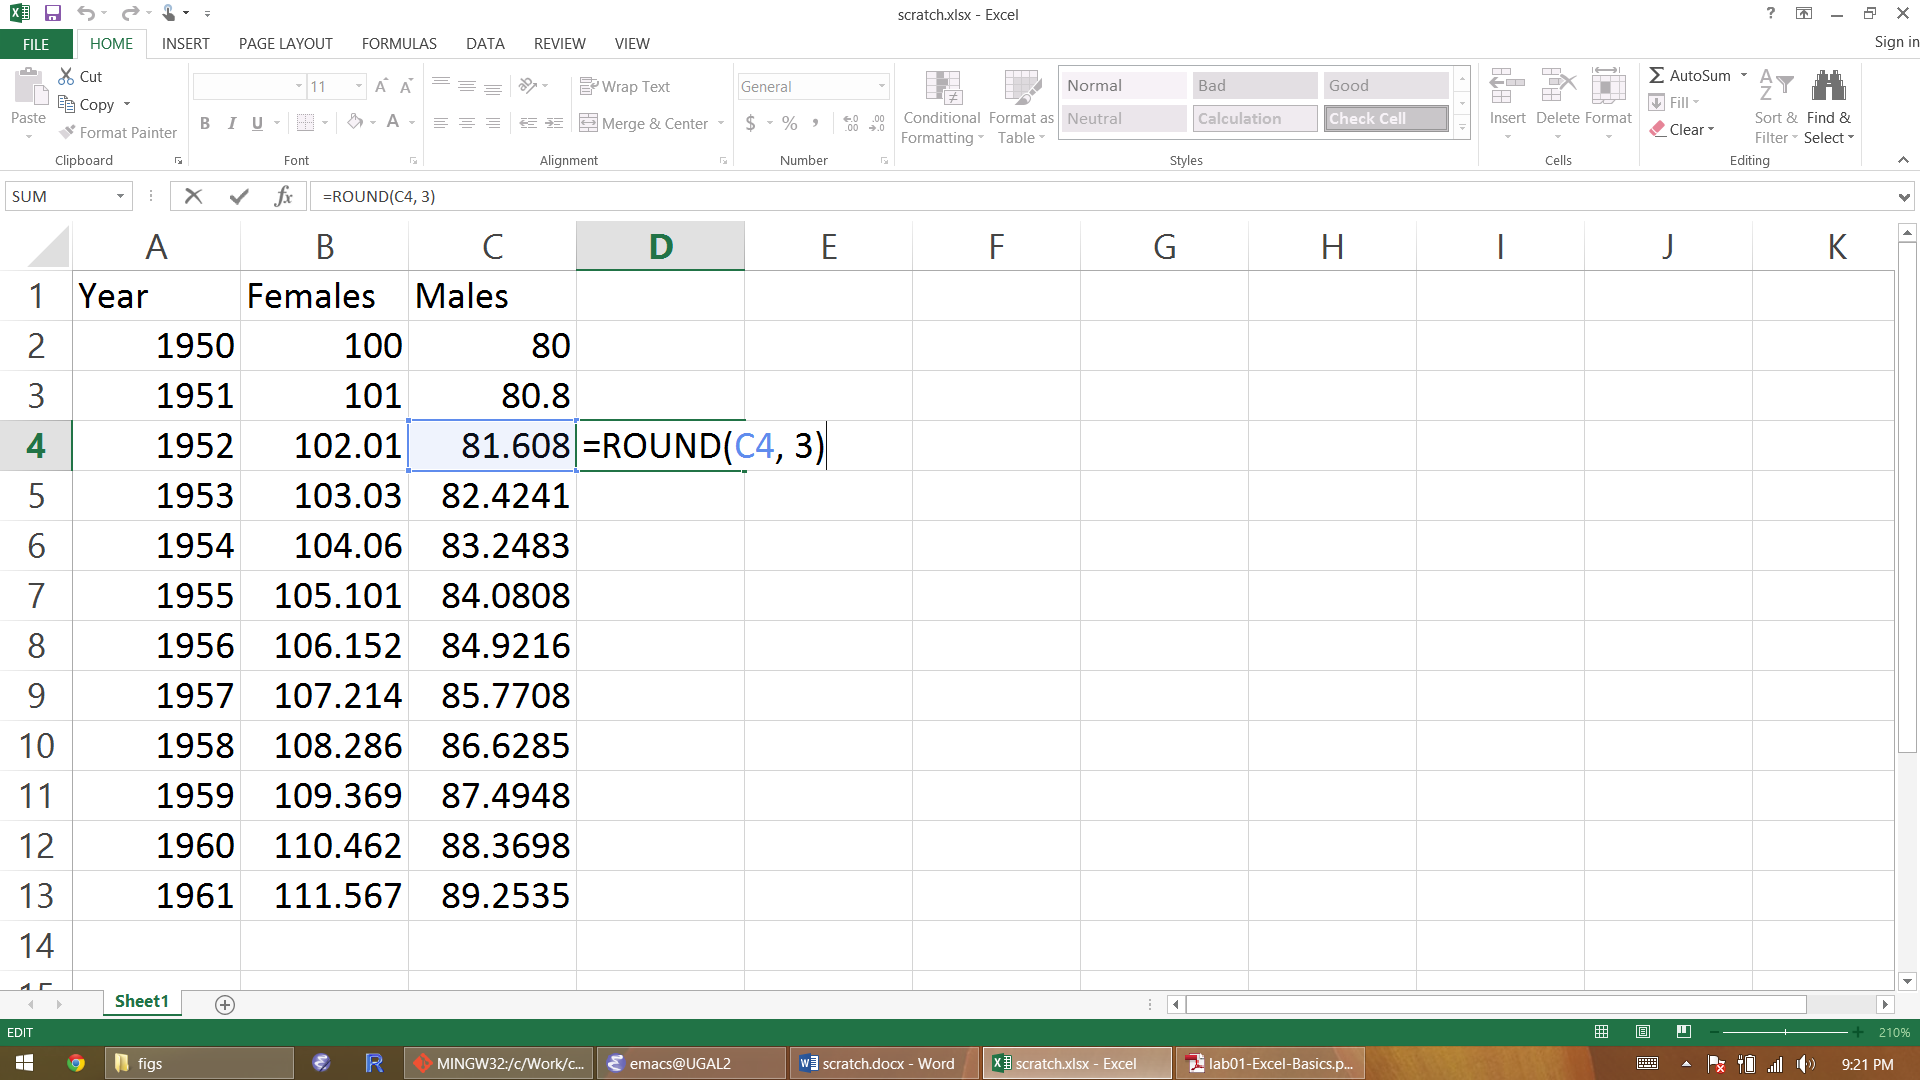
\includegraphics[width=\textwidth]{figs/formula}}
\end{frame}


\section{Graphics}



\begin{frame}
  \frametitle{Graphics}
%  \begin{overprint}
    \fbox{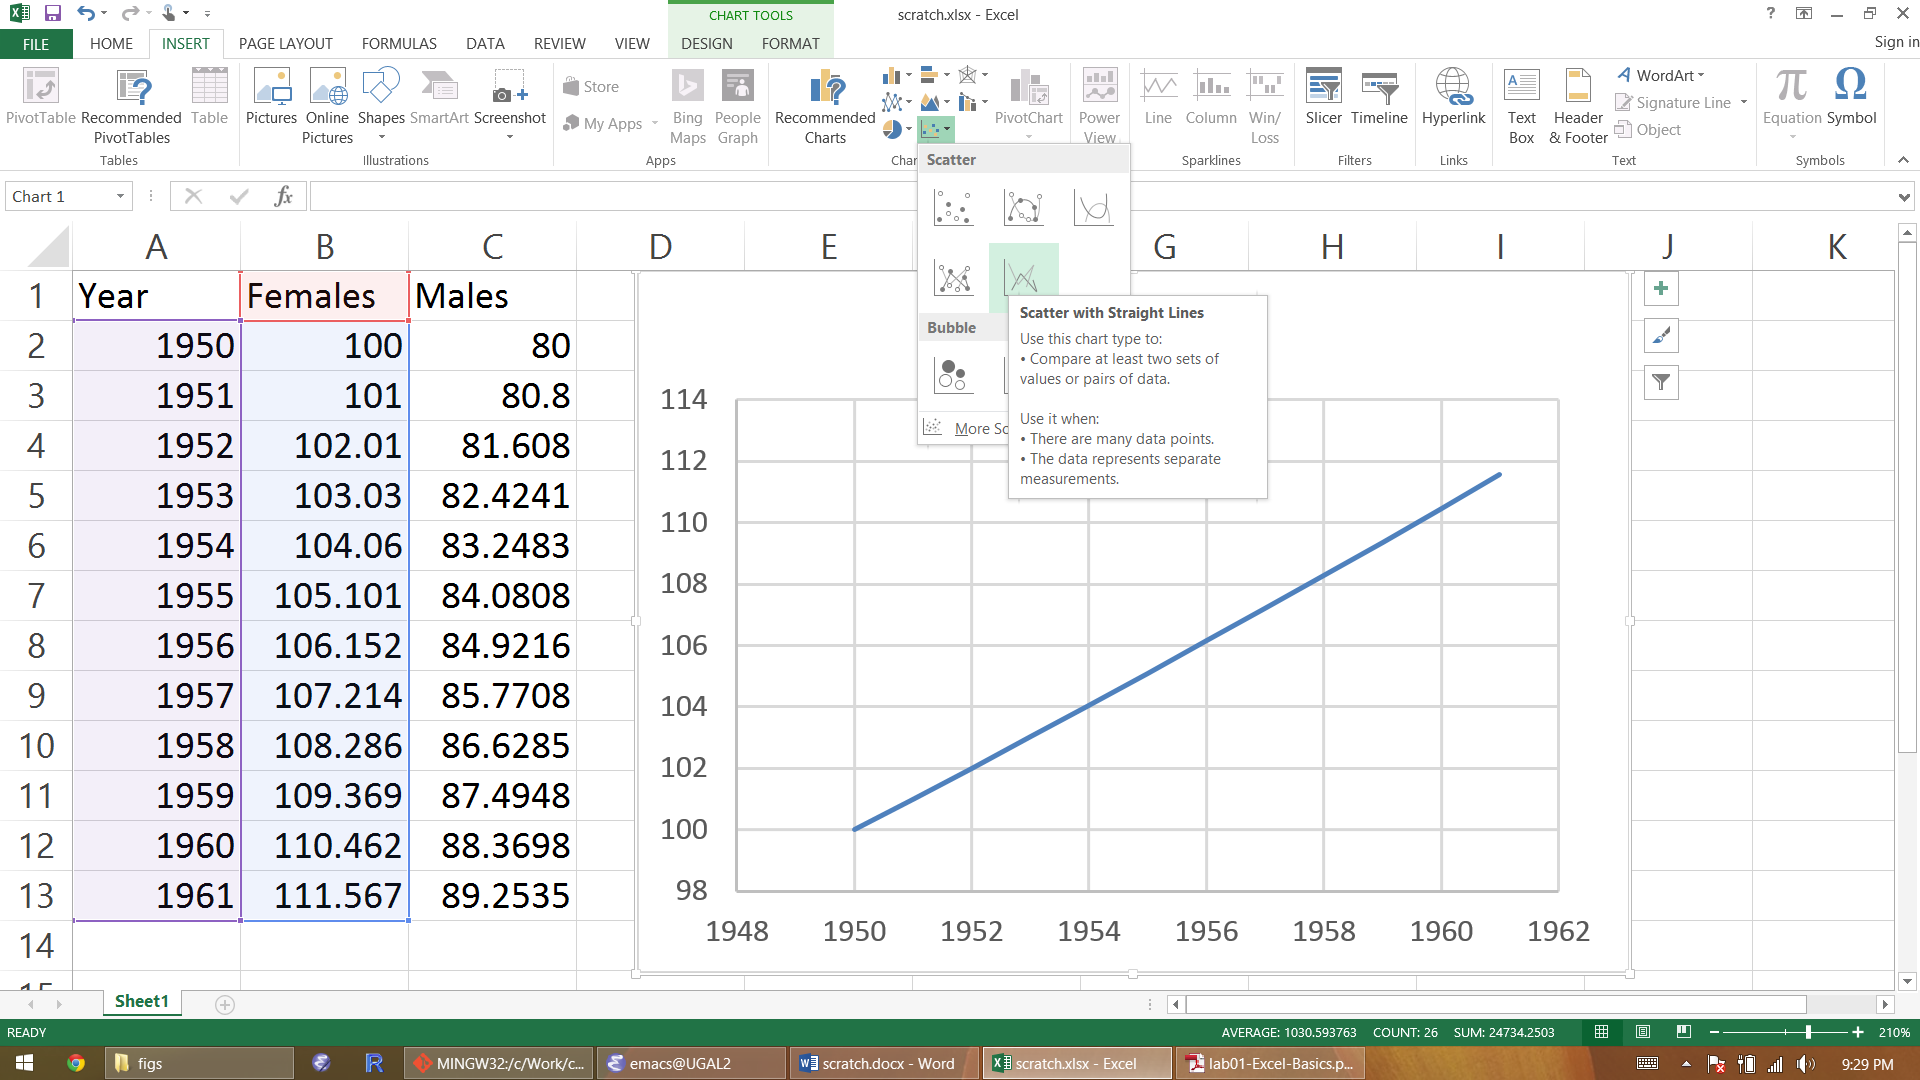
\includegraphics[width=\textwidth]{figs/scatterlines}}
%    \only<2 | handout:0>{\fbox{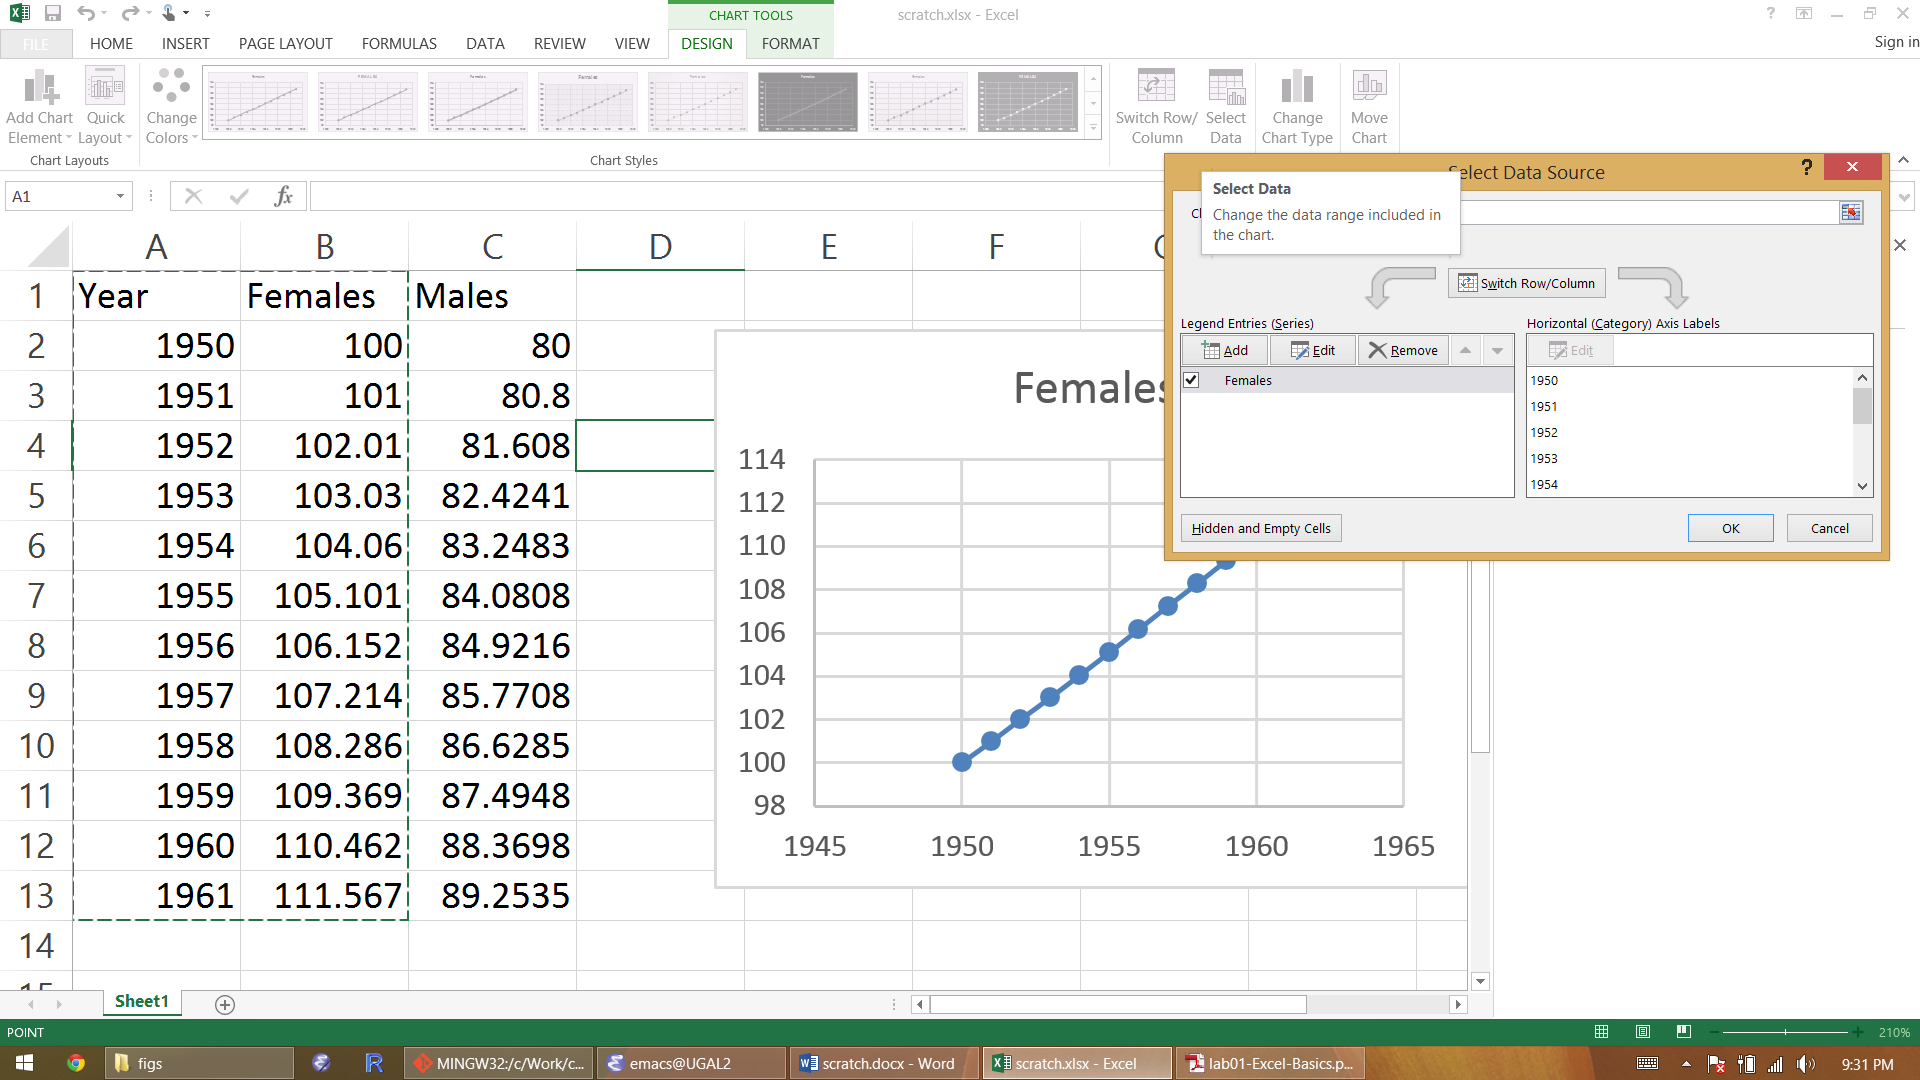
\includegraphics[width=\textwidth]{figs/scatterlines2}}}
%  \end{overprint}
\end{frame}


\begin{frame}
  \frametitle{Graphics}
  \only<1>{\fbox{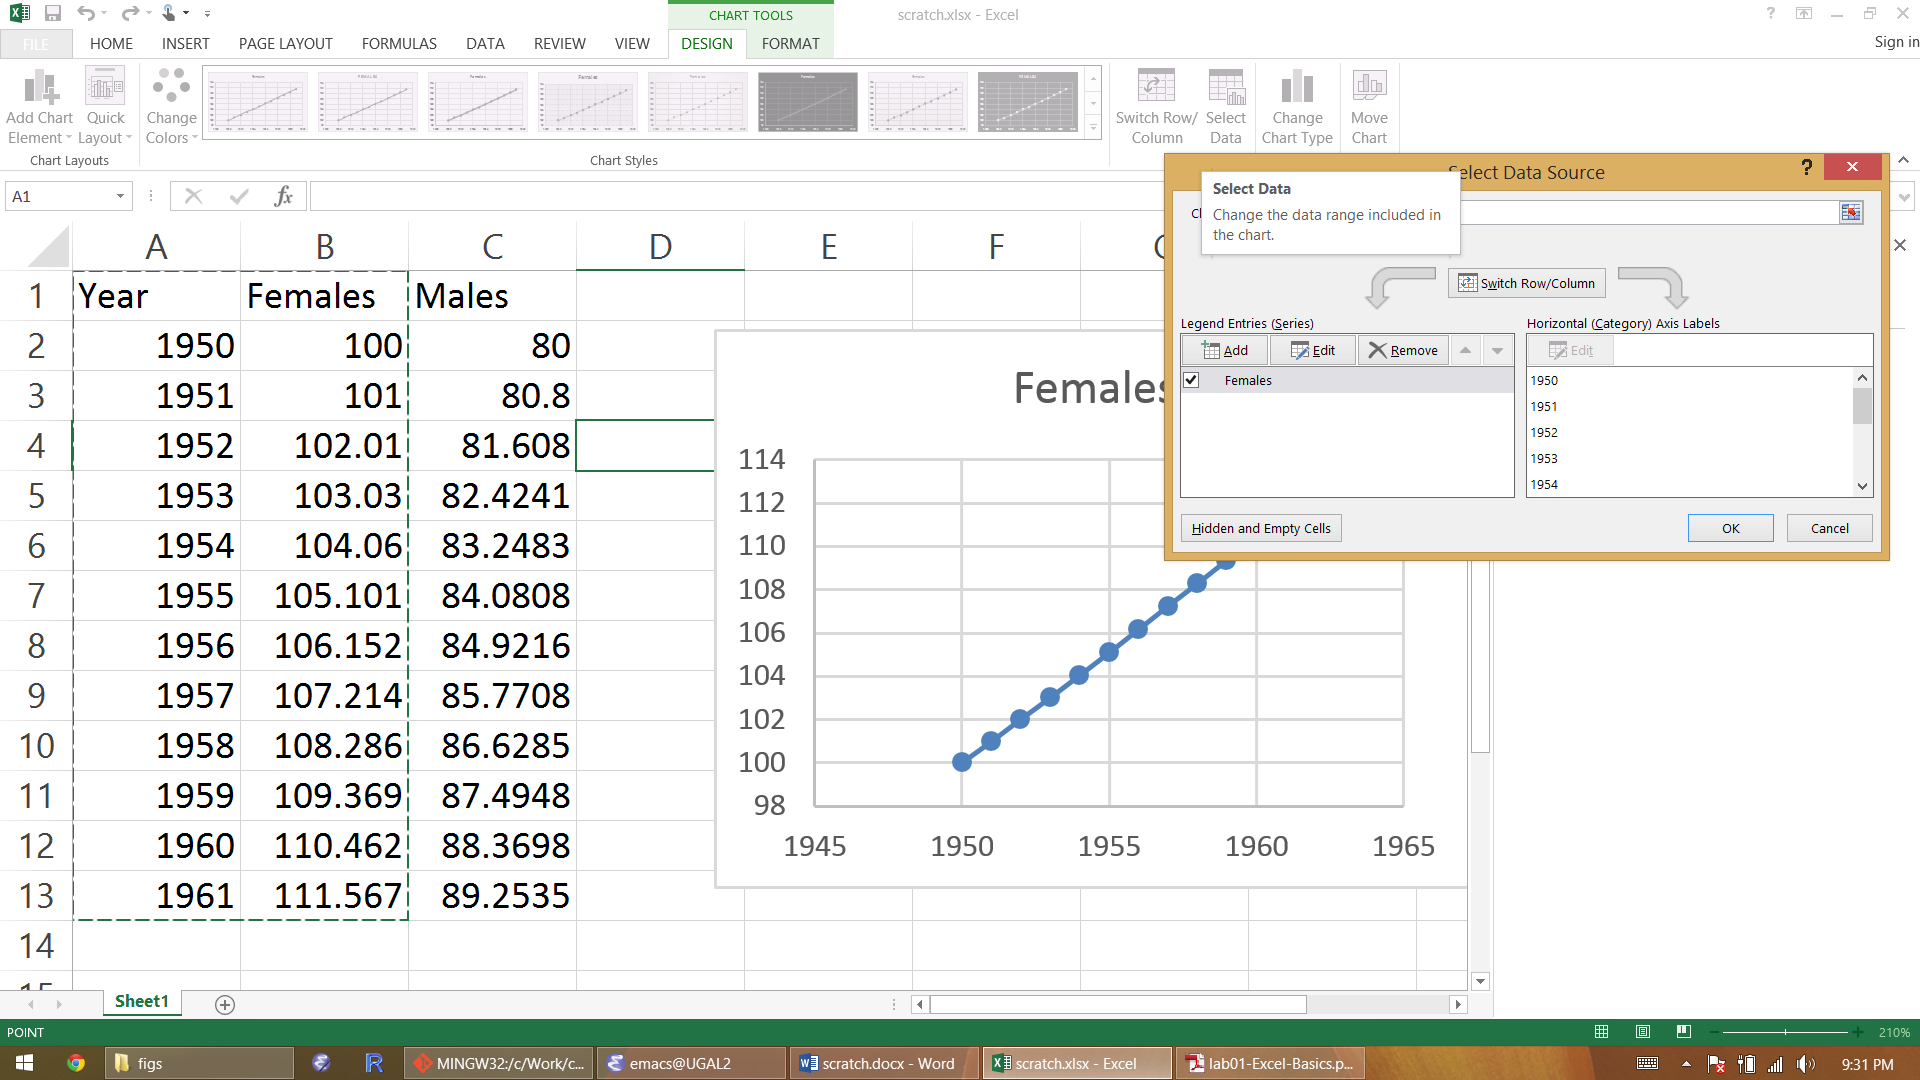
\includegraphics[width=\textwidth]{figs/scatterlines2}}}
  \only<2>{\fbox{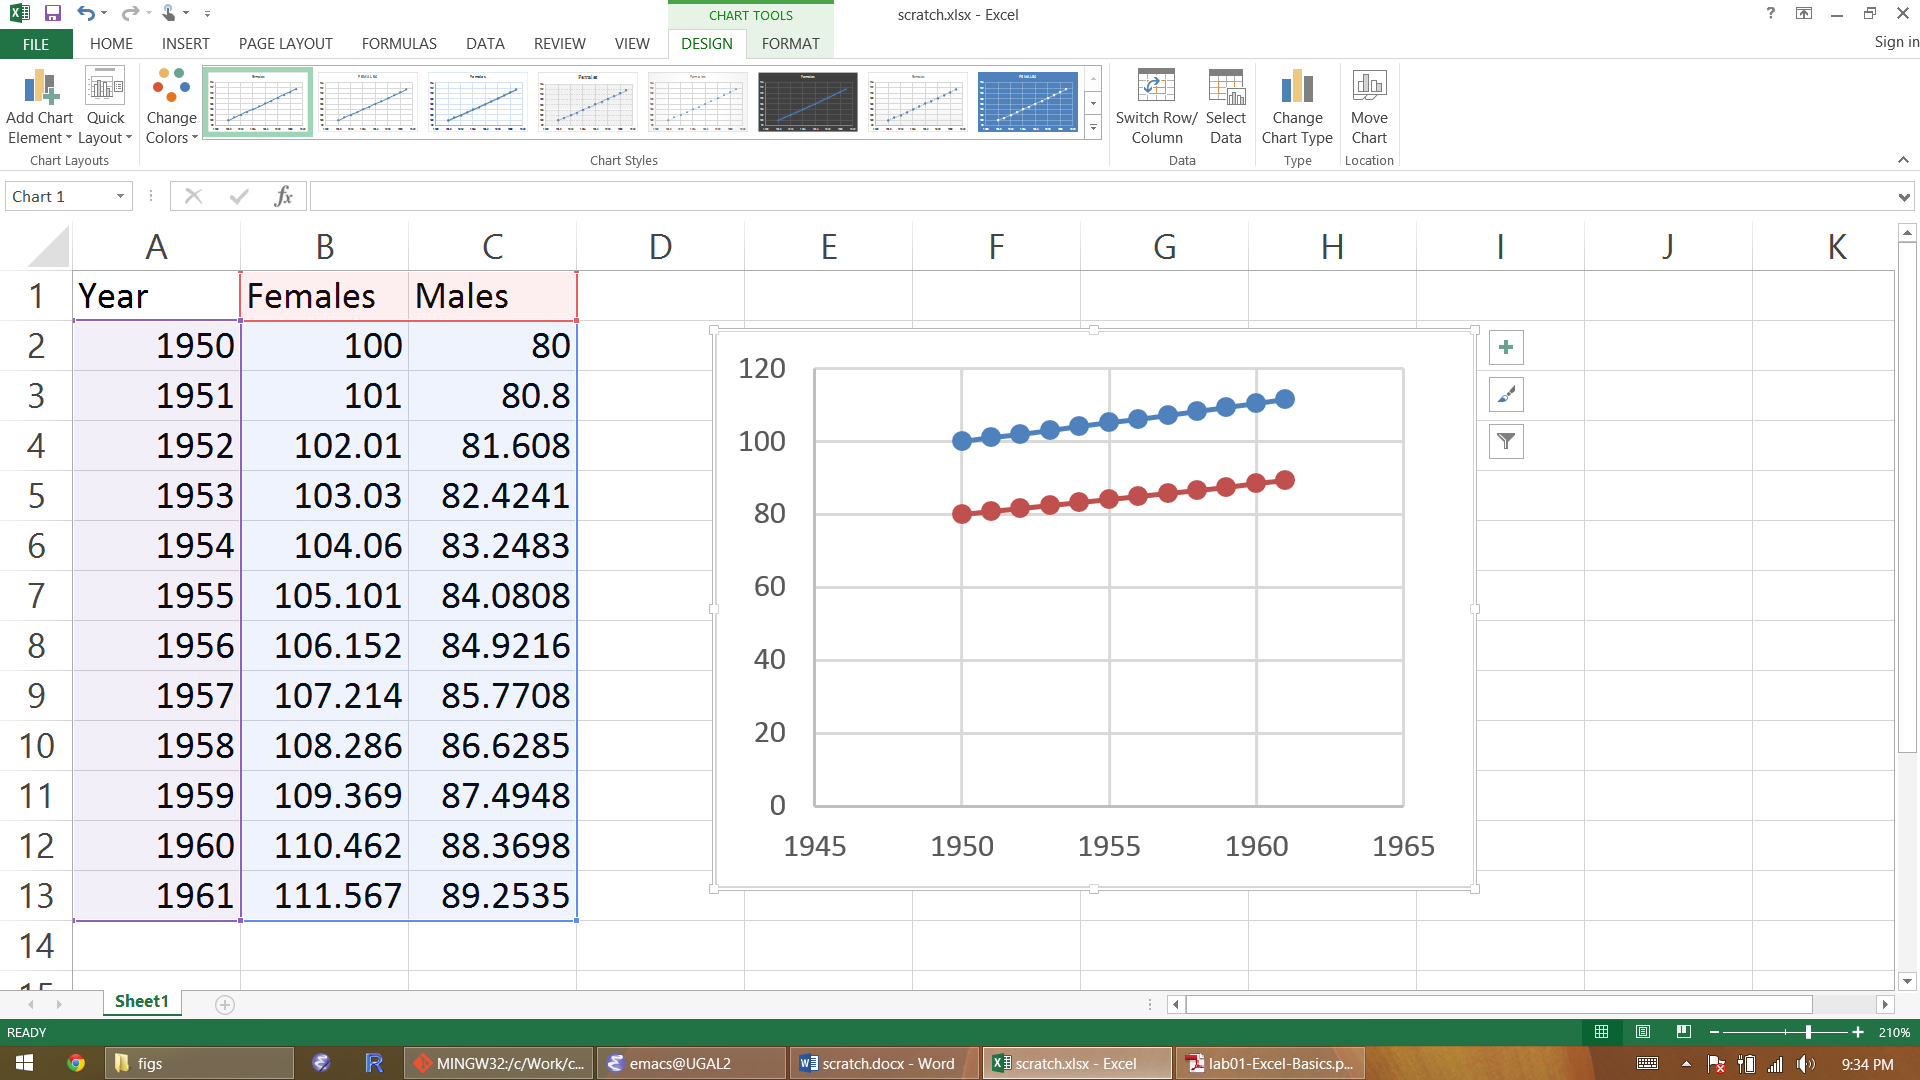
\includegraphics[width=\textwidth]{figs/scatterlines3}}}
  \begin{center}
    Add a line for males
  \end{center}
\end{frame}


% \begin{frame}
%   \frametitle{Add Headings}
%   \only<1>{\fbox{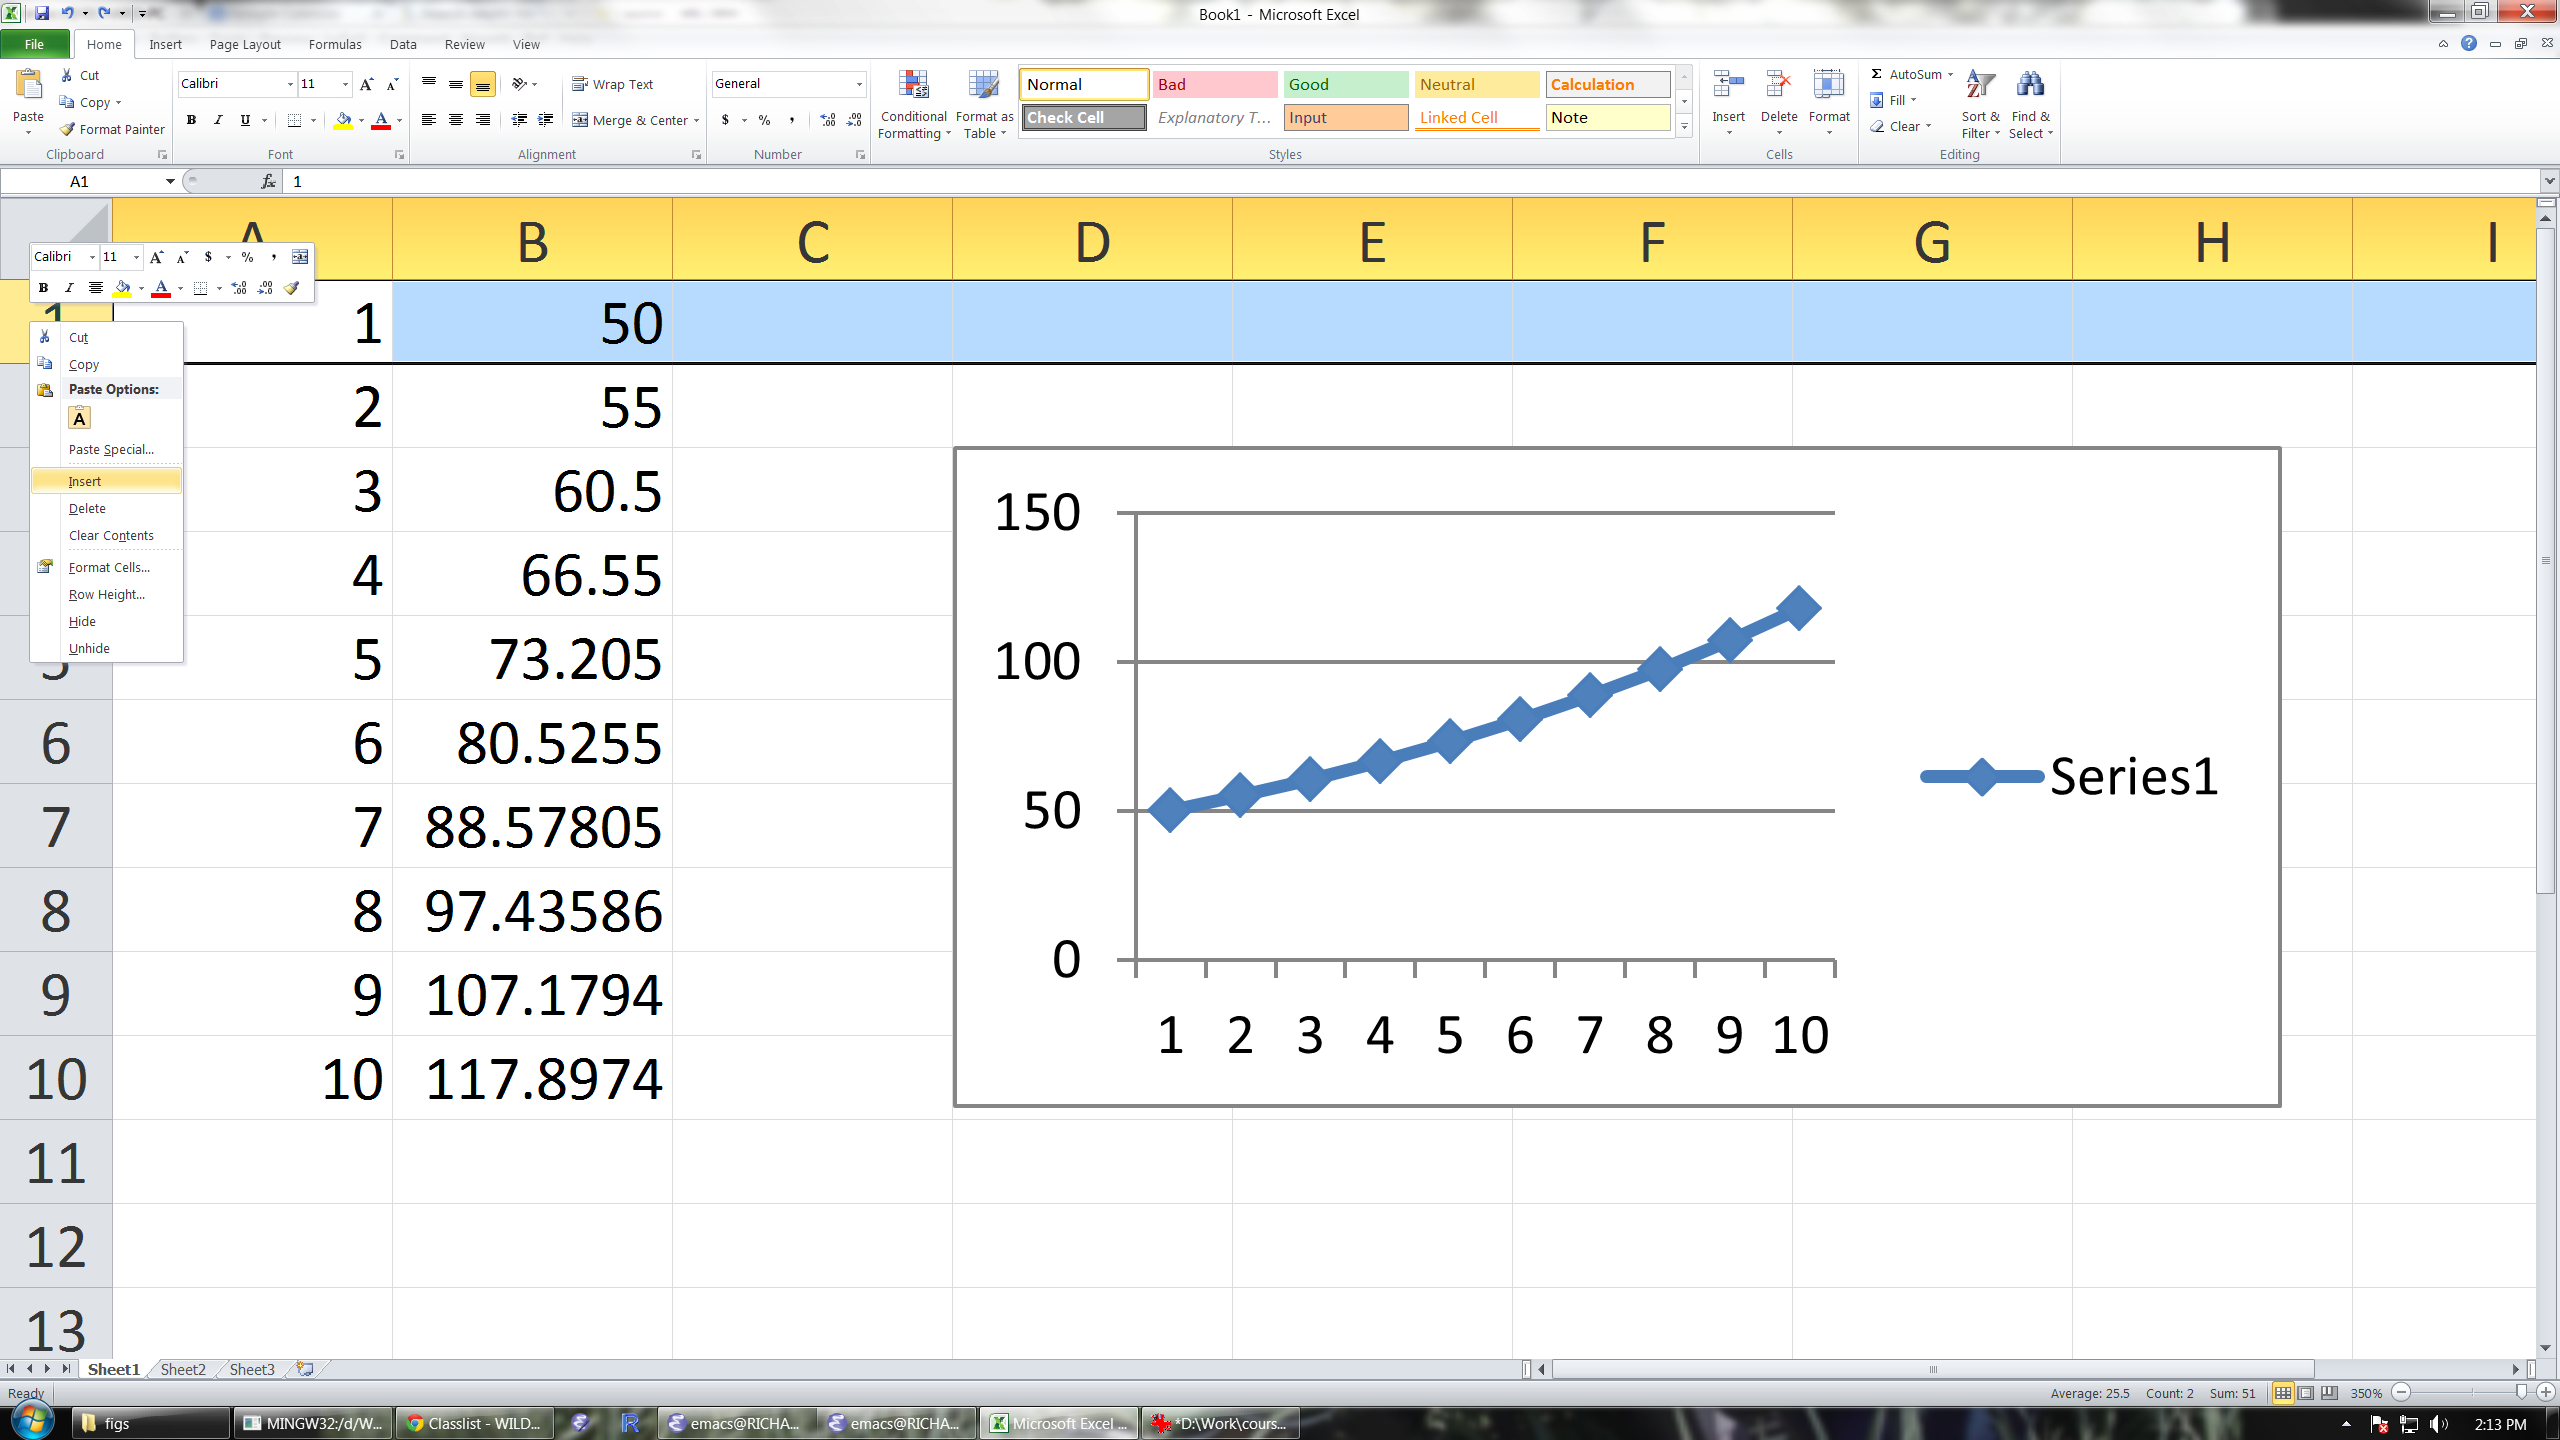
\includegraphics[width=\textwidth]{figs/headings}}}
%   \only<2>{\fbox{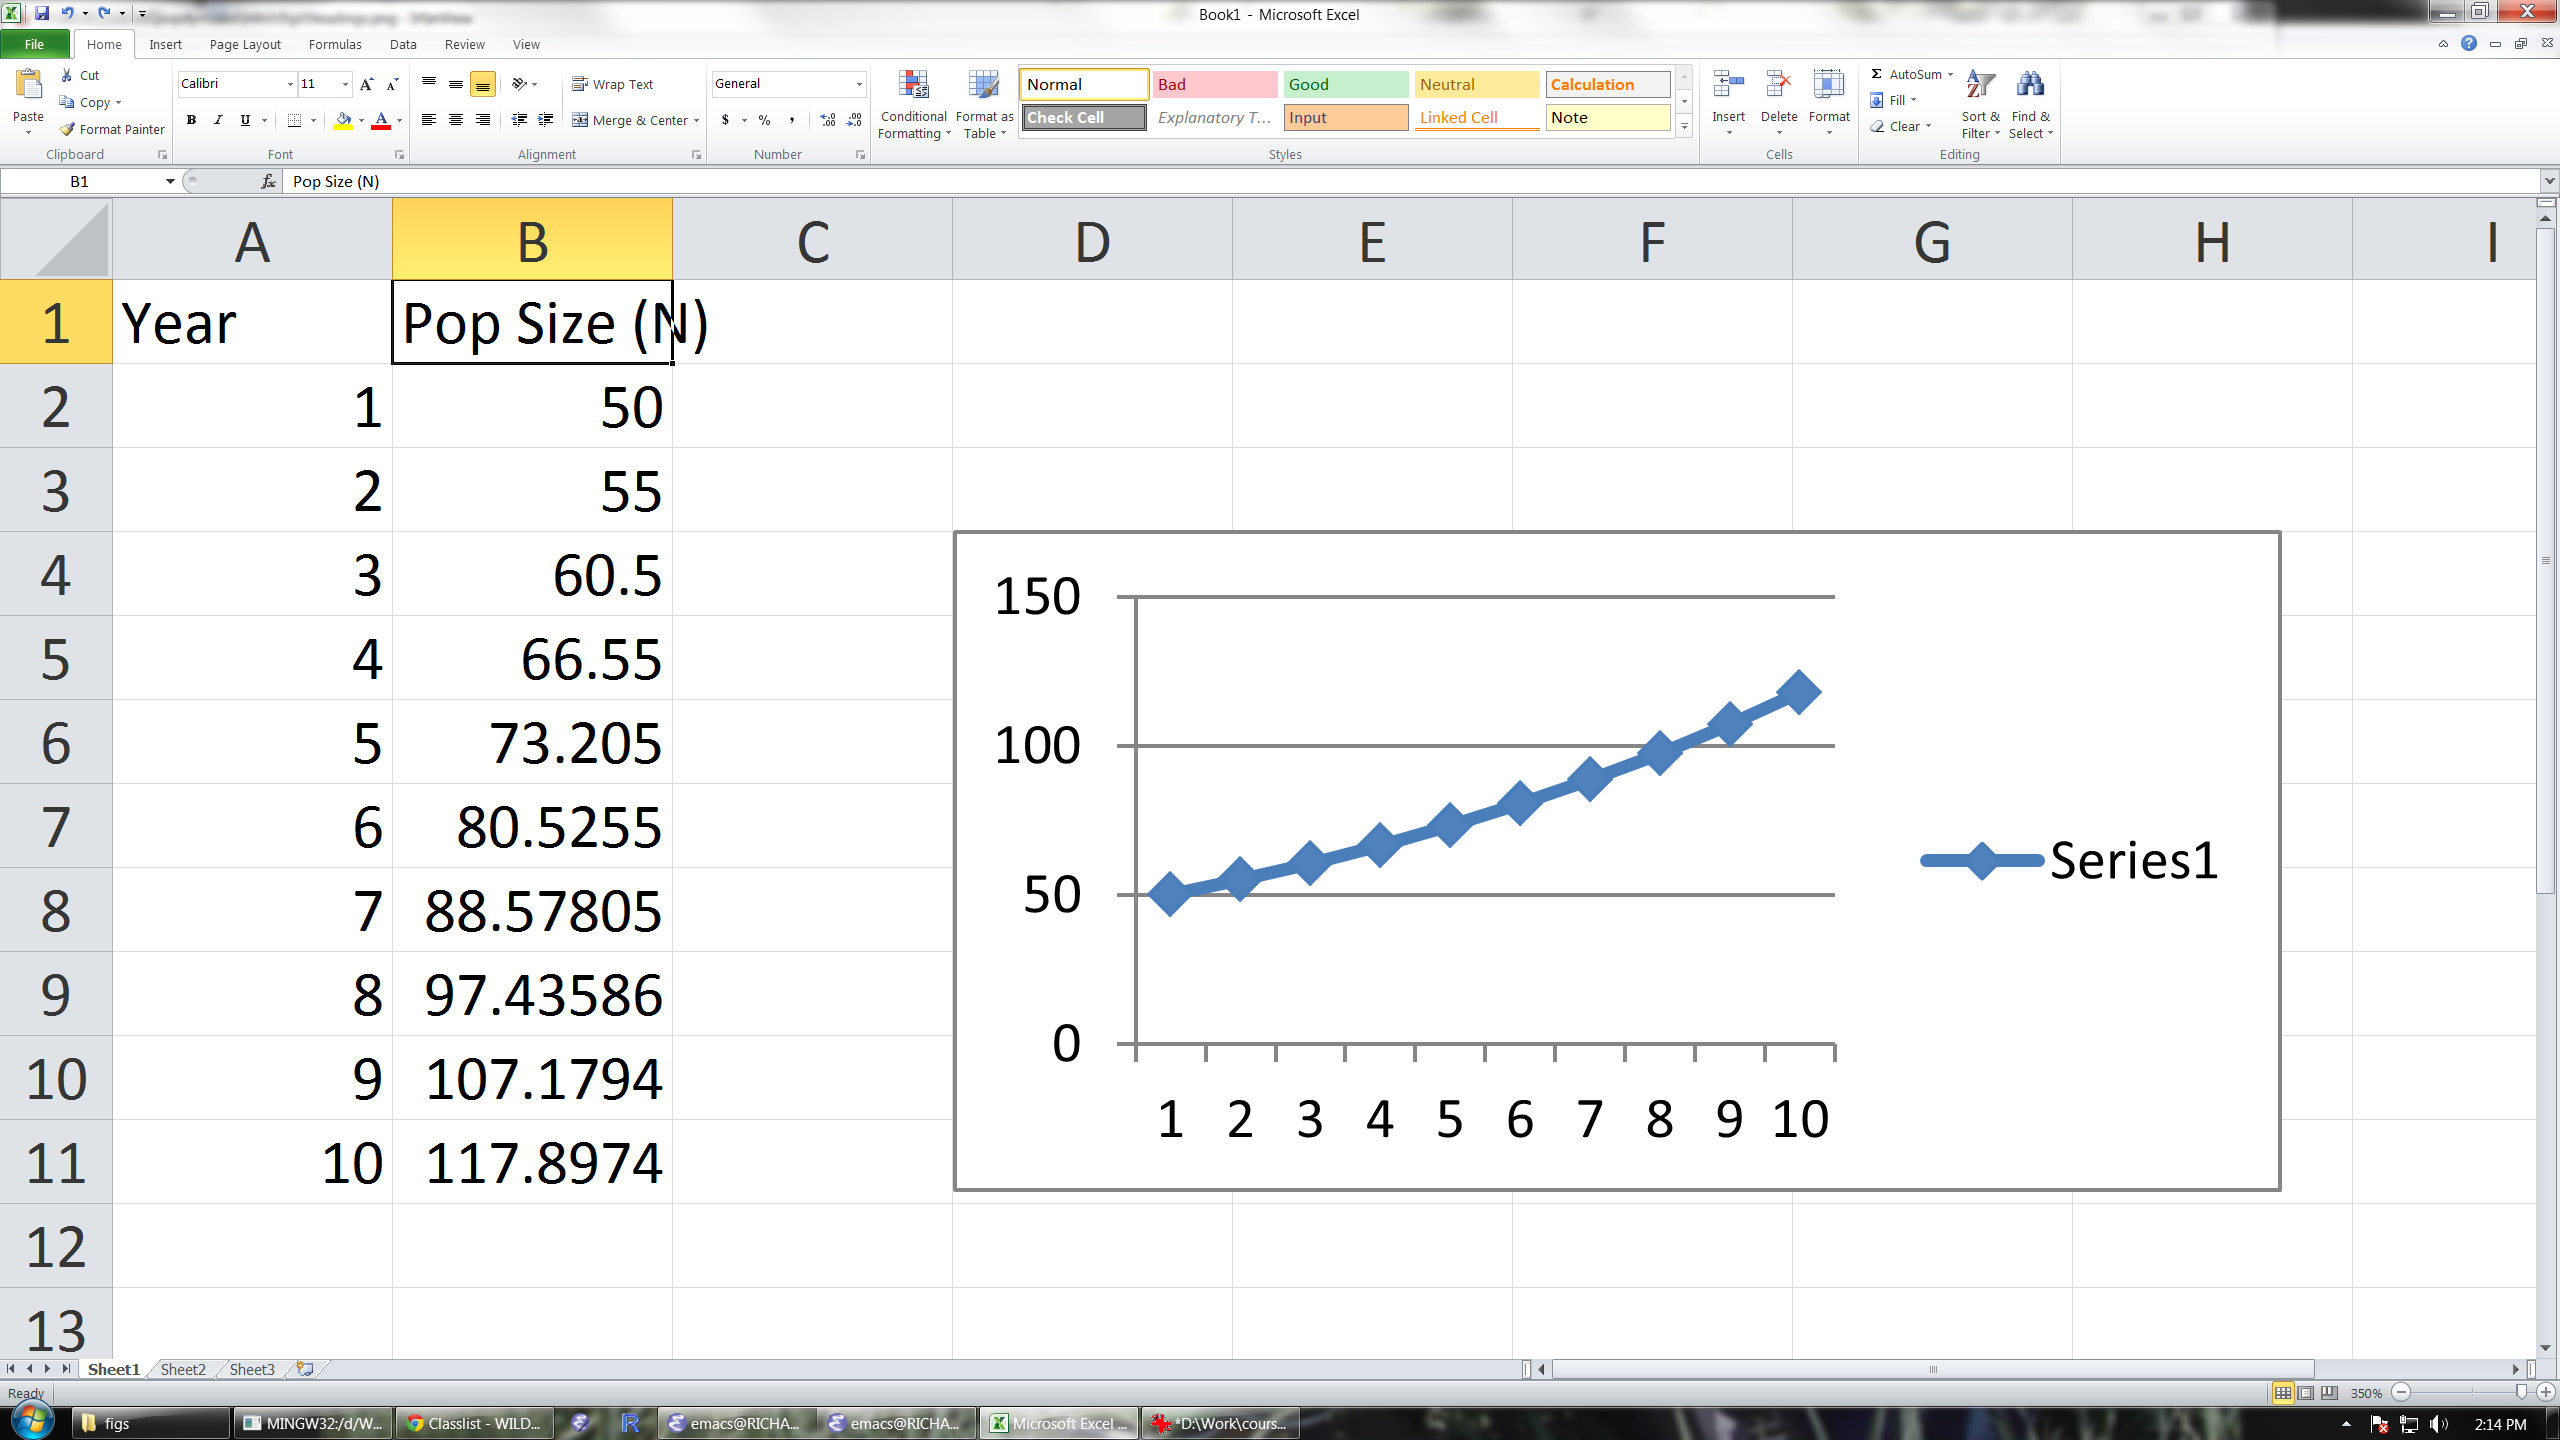
\includegraphics[width=\textwidth]{figs/headings2}}}
% \end{frame}



\begin{frame}
  \frametitle{Customize}
%  \begin{overprint}
    \only<1>{\fbox{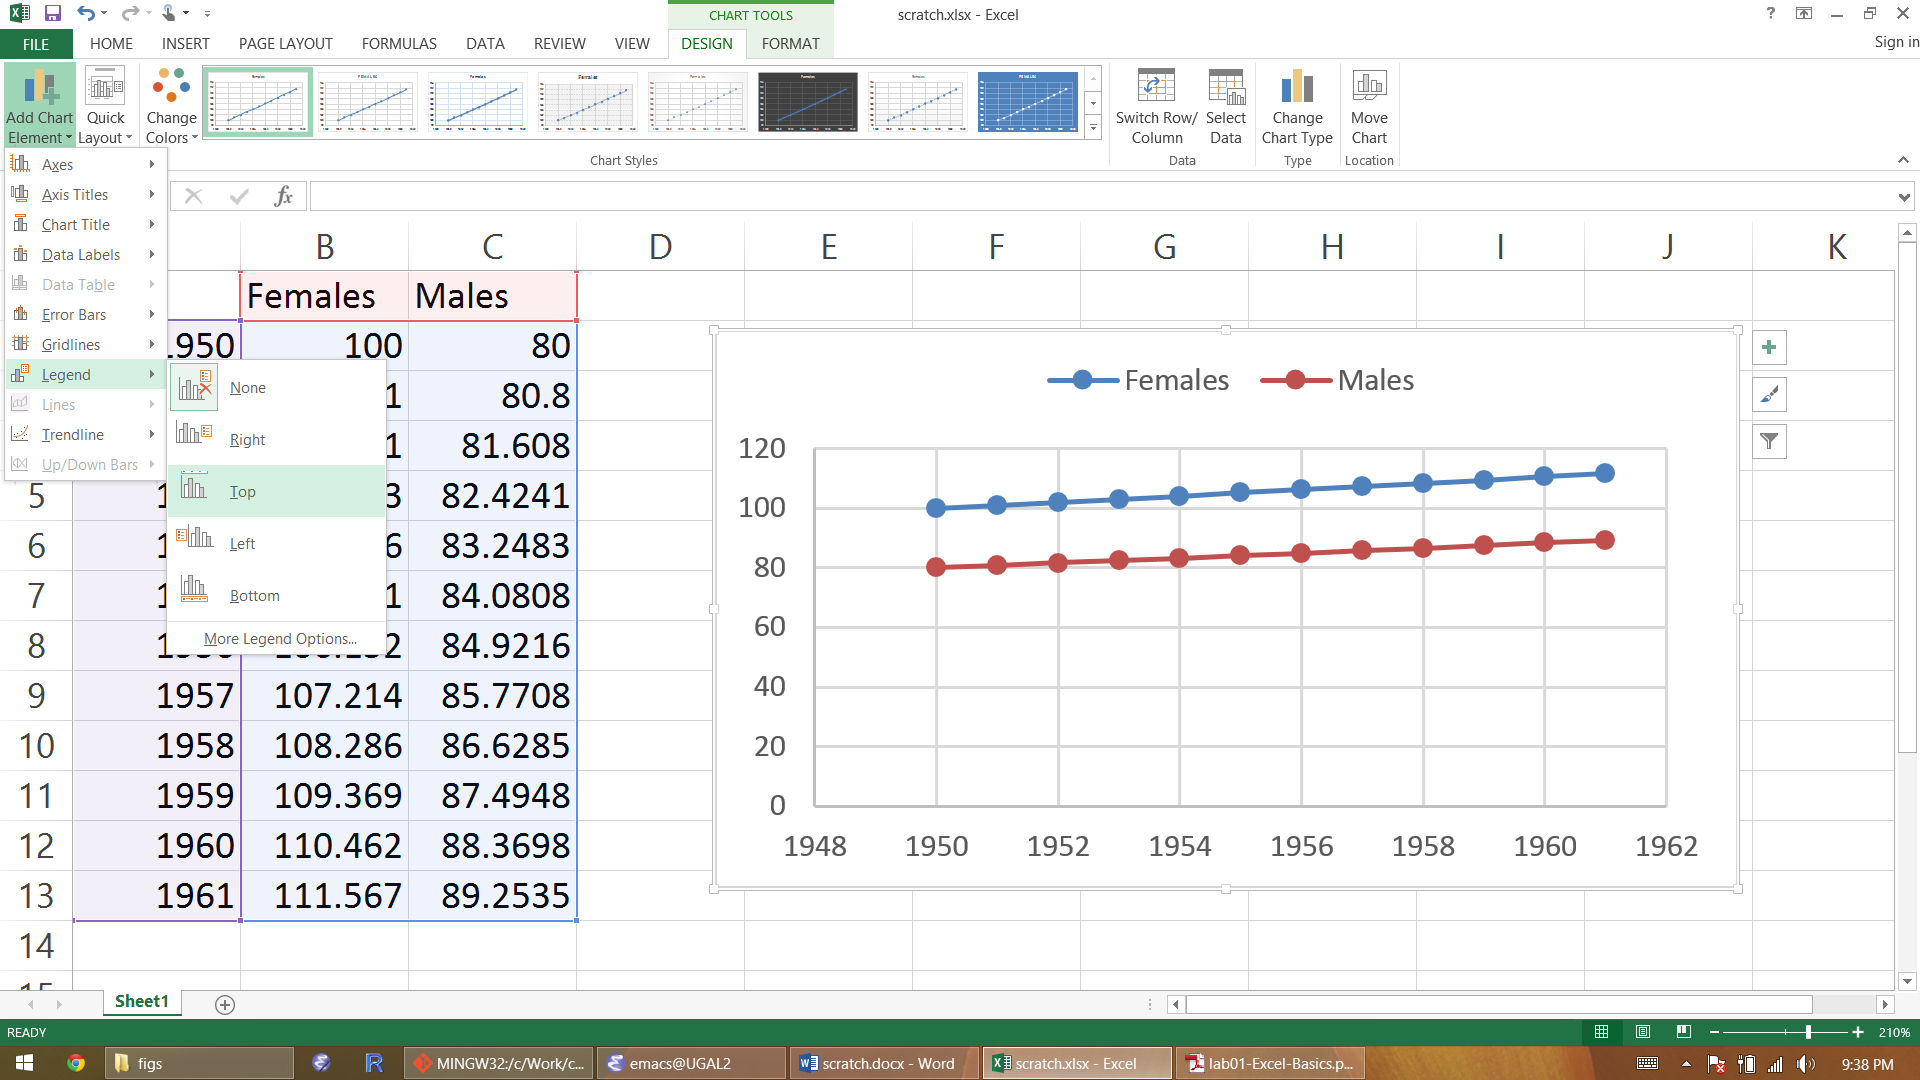
\includegraphics[width=\textwidth]{figs/customize}}}
%    \only<2 | handout:0>{\fbox{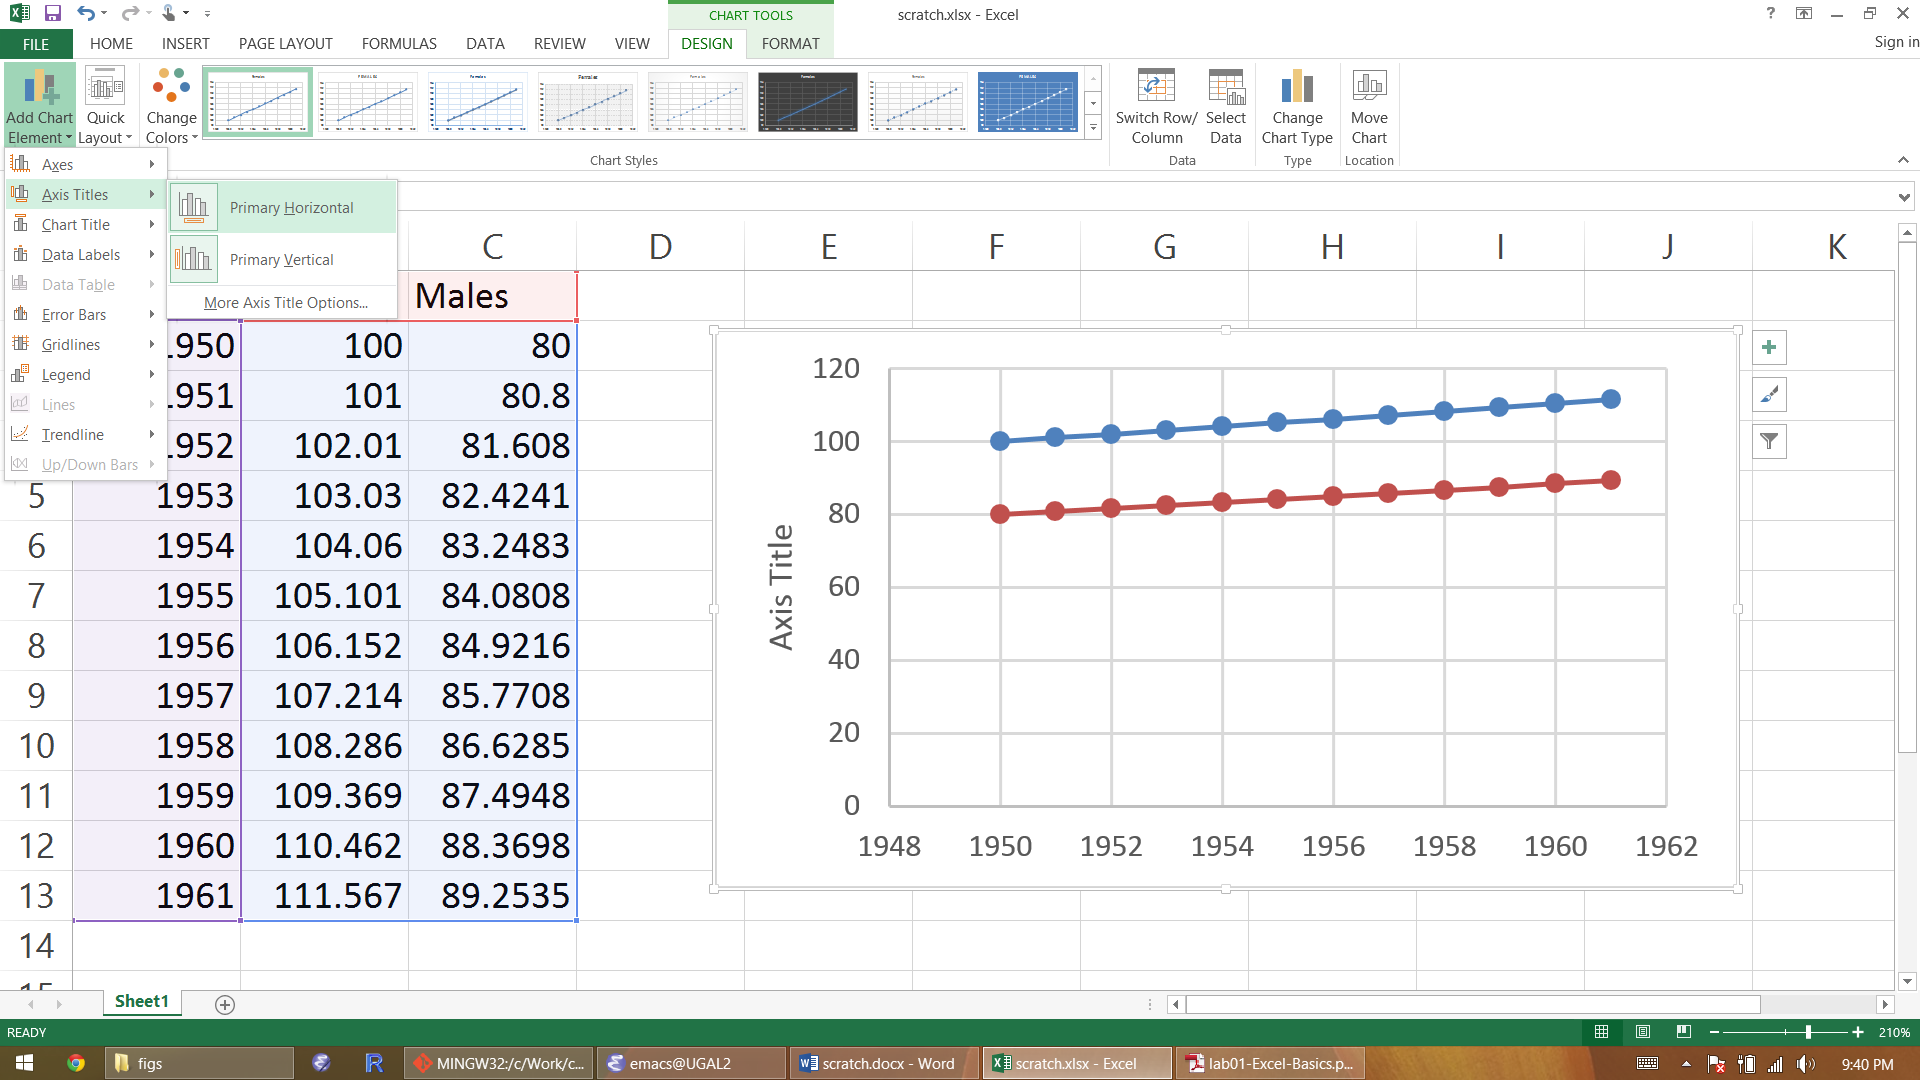
\includegraphics[width=\textwidth]{figs/customize2}}}
%  \end{overprint}
    \begin{center}
      Add legend
    \end{center}
\end{frame}



\begin{frame}
  \frametitle{Customize}
    \fbox{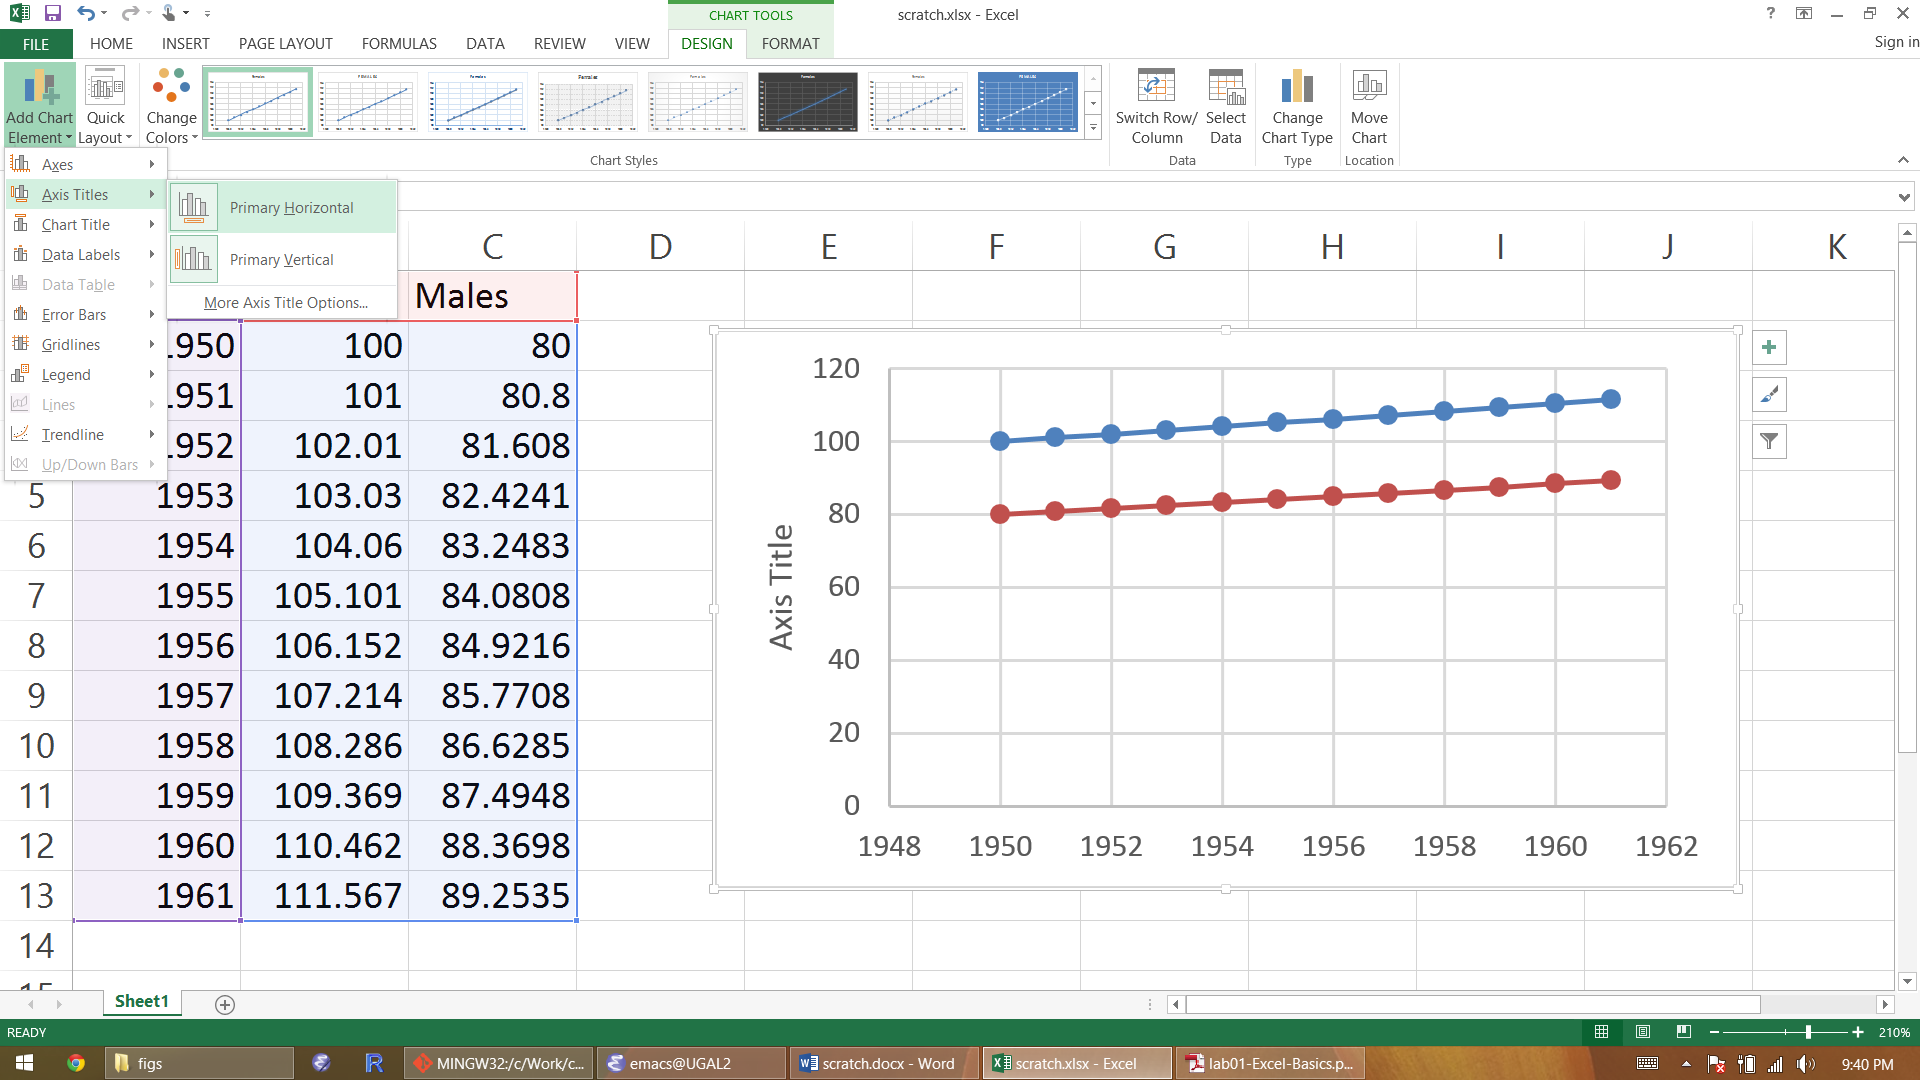
\includegraphics[width=\textwidth]{figs/customize2}}
    \begin{center}
      Add axis labels
    \end{center}
\end{frame}



\begin{frame}
  \frametitle{Customize}
    \fbox{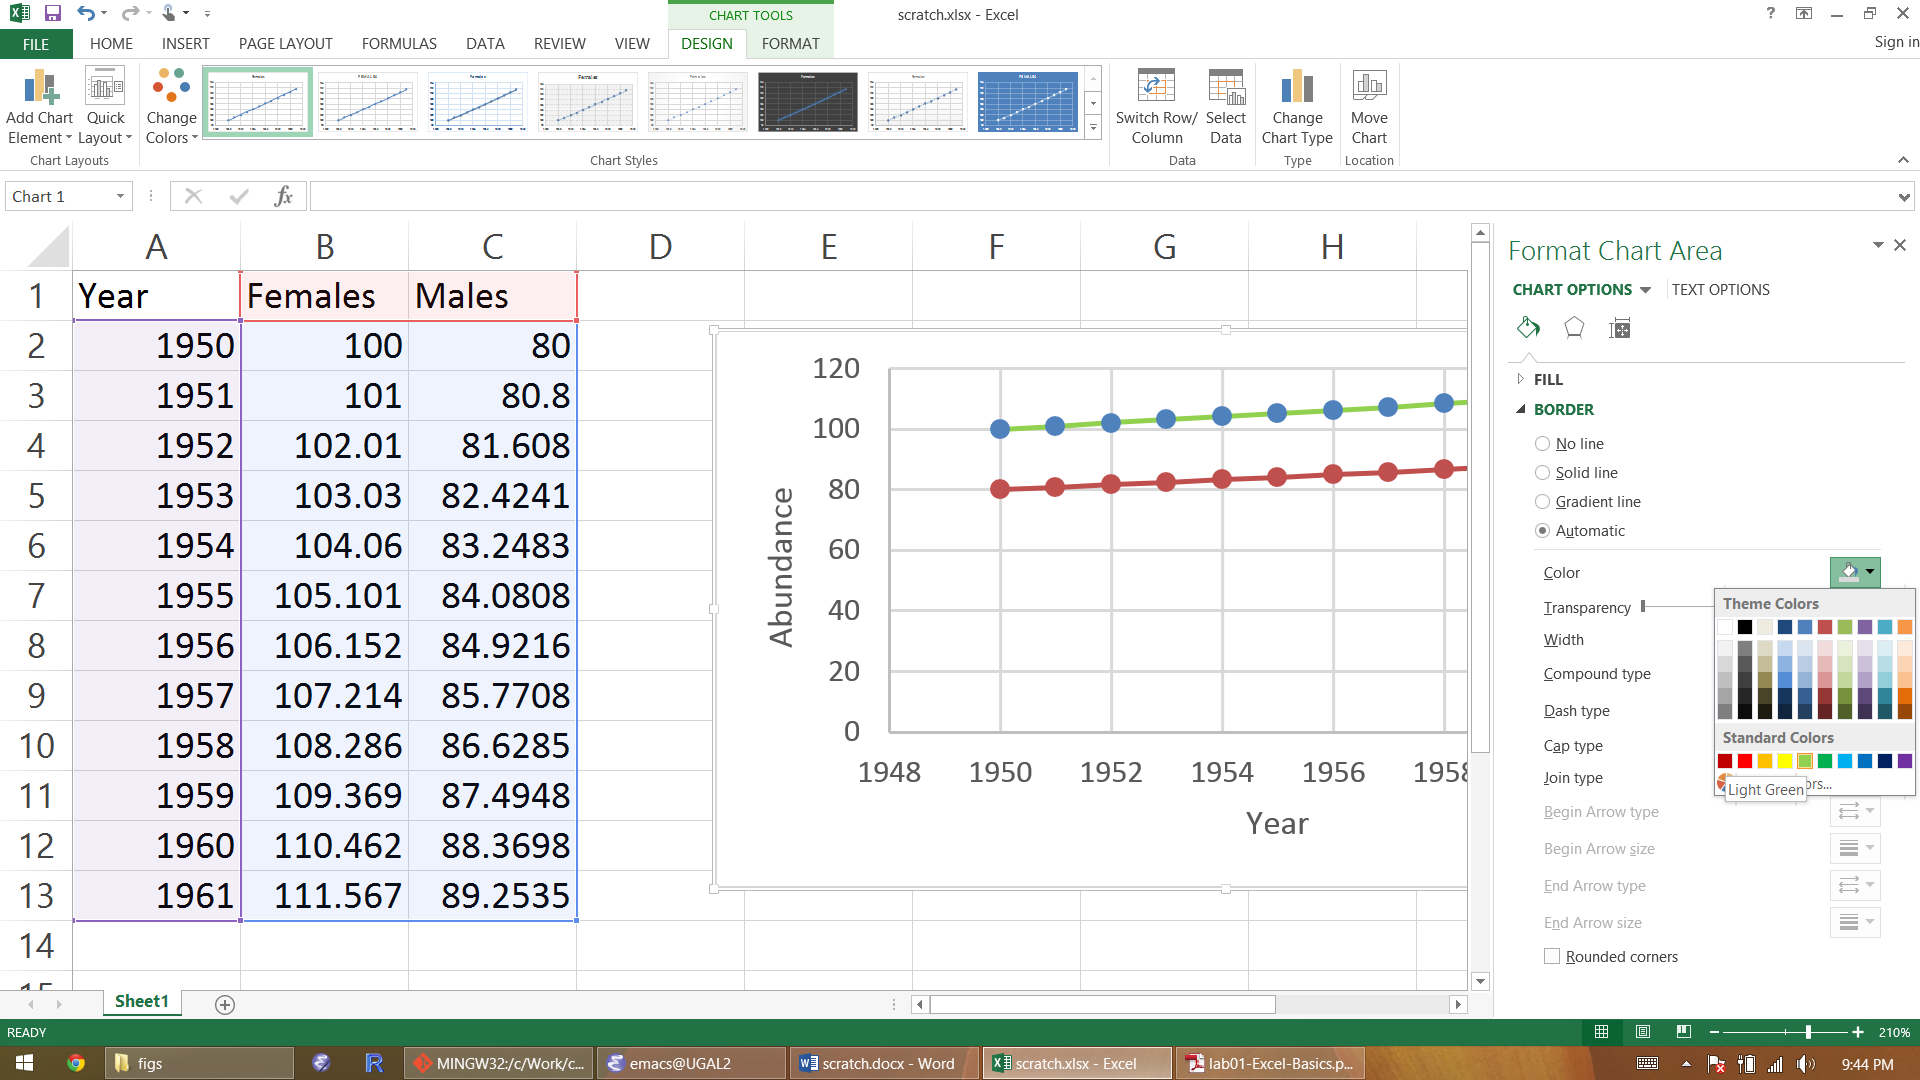
\includegraphics[width=\textwidth]{figs/customize3}}
    \begin{center}
      Change line color
    \end{center}
\end{frame}



% \section{In-class exercise}



% \begin{frame}
%   \frametitle{In-class exercise}
%   \fbox{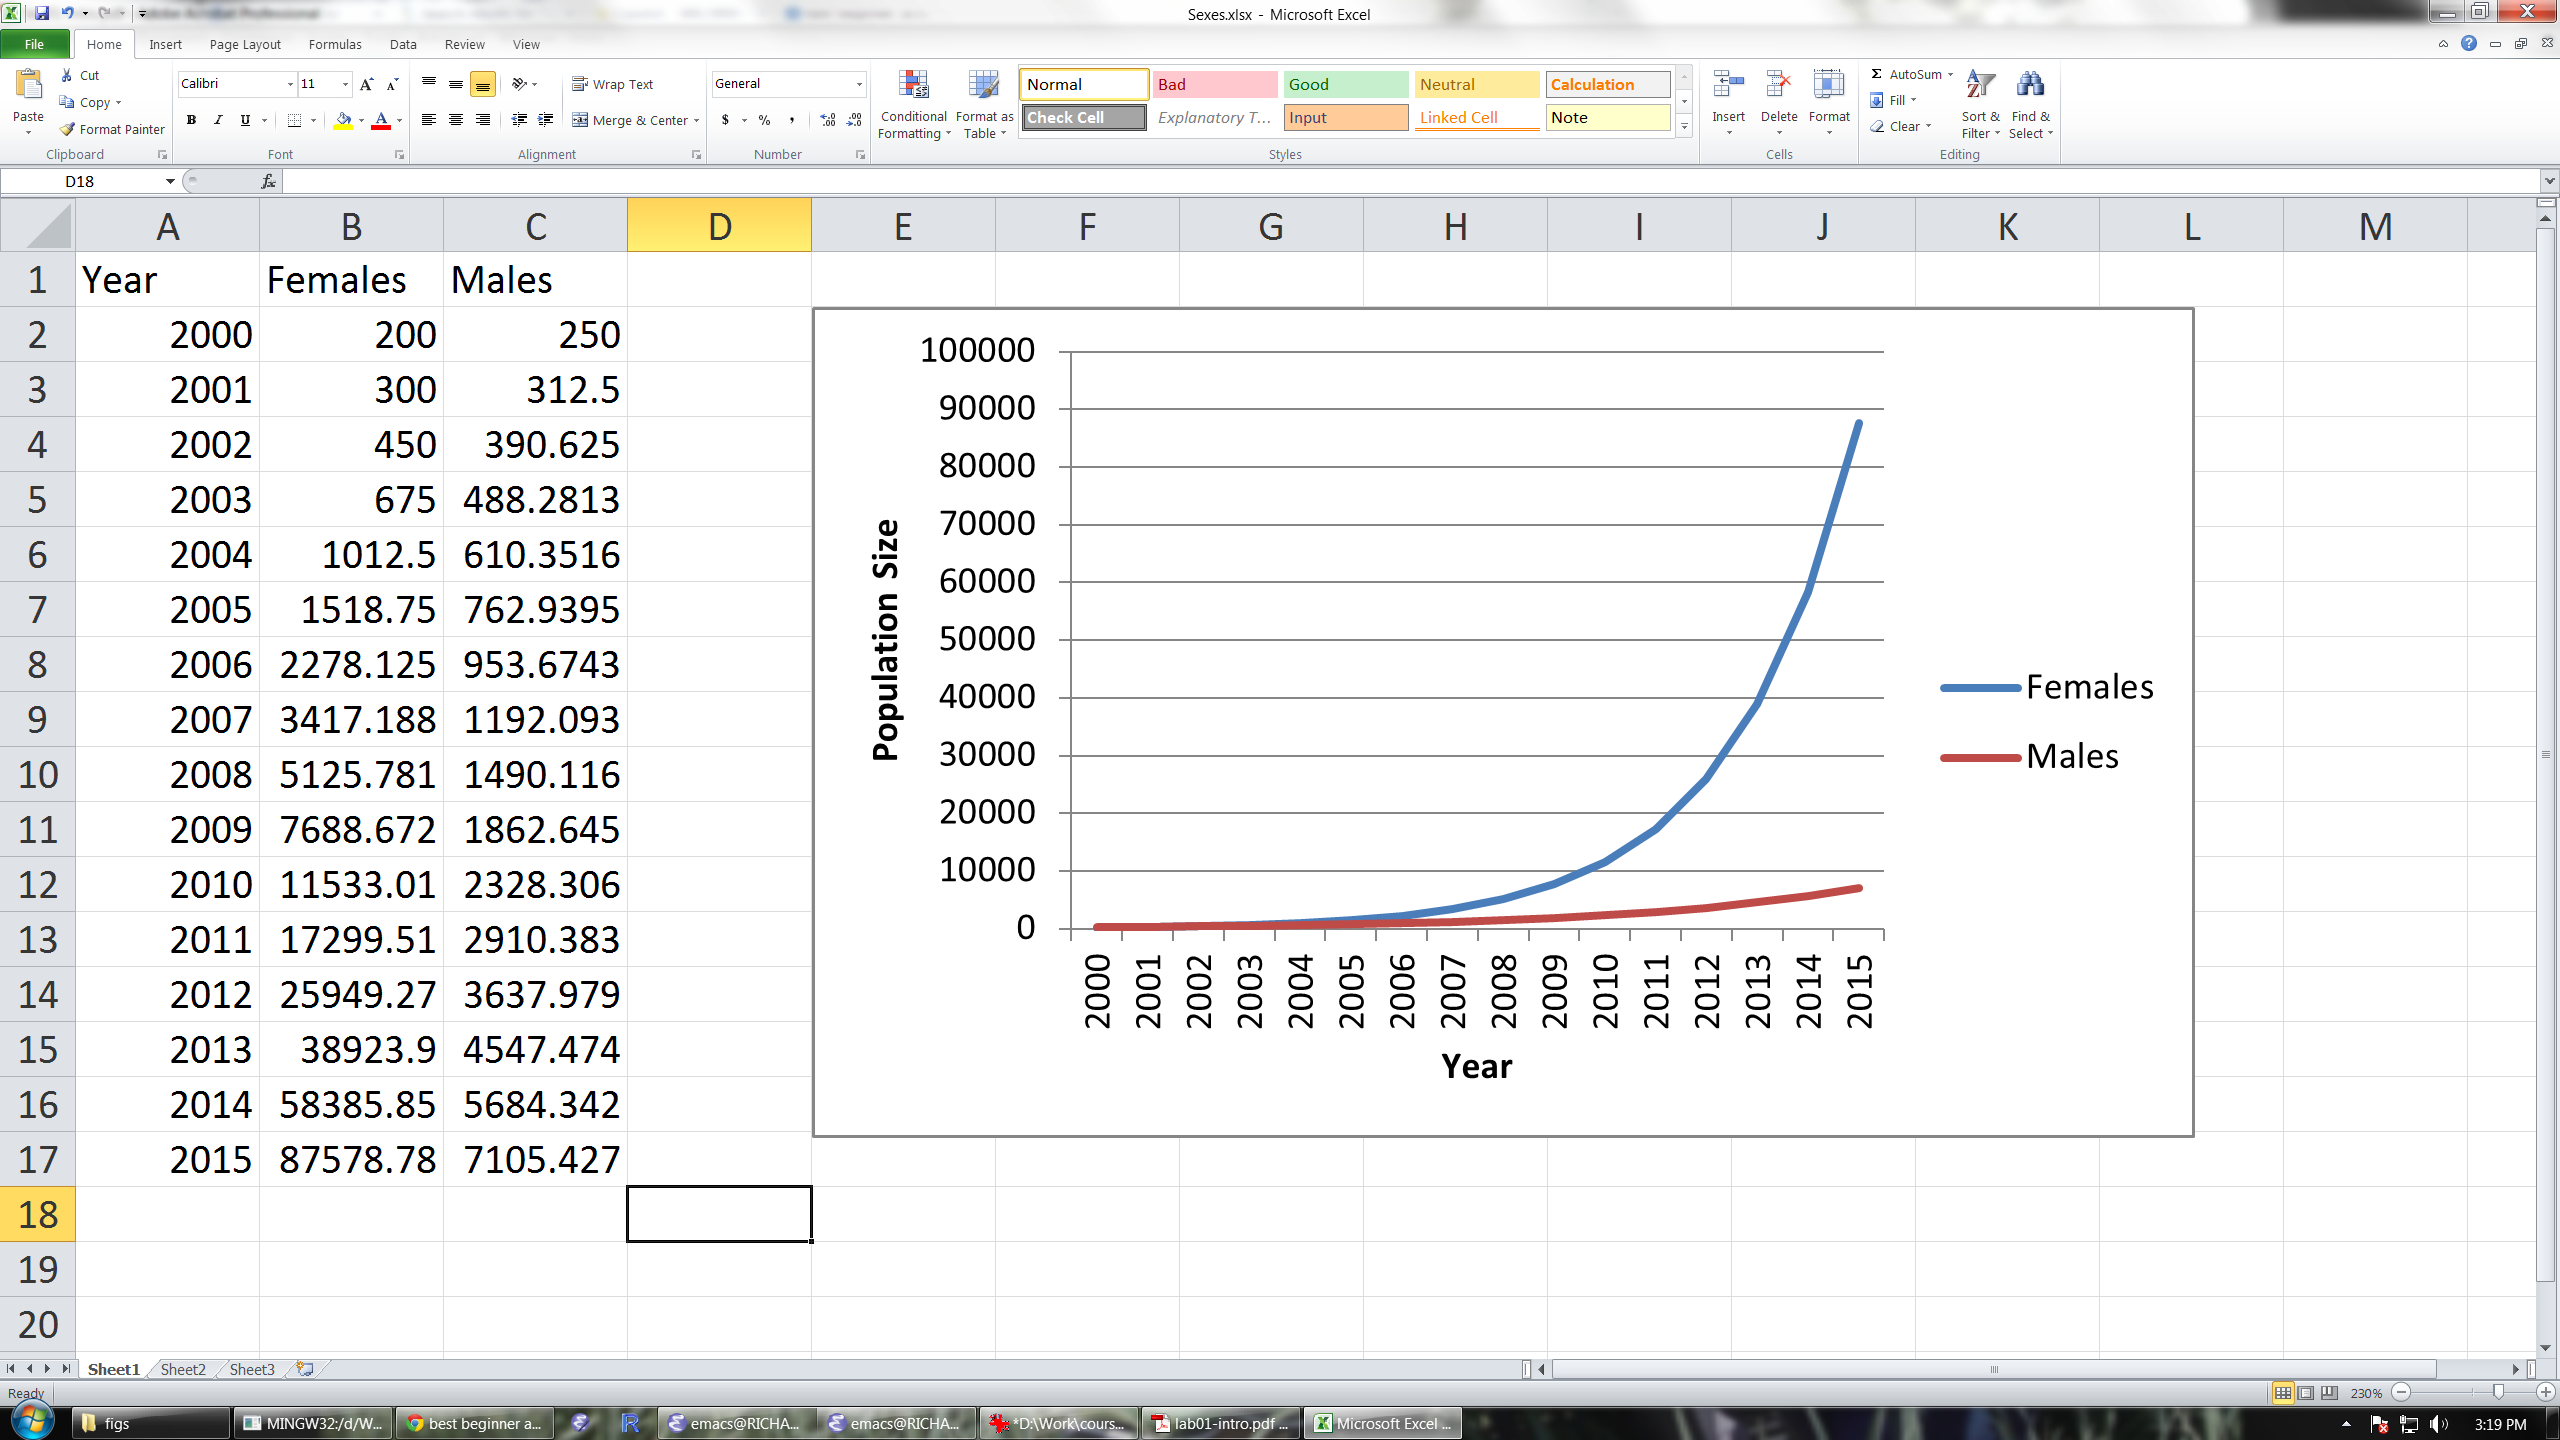
\includegraphics[width=\textwidth]{figs/inclass1}}
% \end{frame}




% \section{Assignment}


% \begin{frame}
%   \frametitle{Assignment}
%   \small
%   \begin{enumerate}[(1)]
%     \item Create an Excel file and name it
%       ``Yourlastname-yourfirstname''
%     \item Create the sheet shown below using techniques covered in
%       this lab (don't just type the numbers in)
%     \item Upload to ELC Dropbox (\url{elcnew.uga.edu})
%   \end{enumerate}
%   \begin{center}
%     \fbox{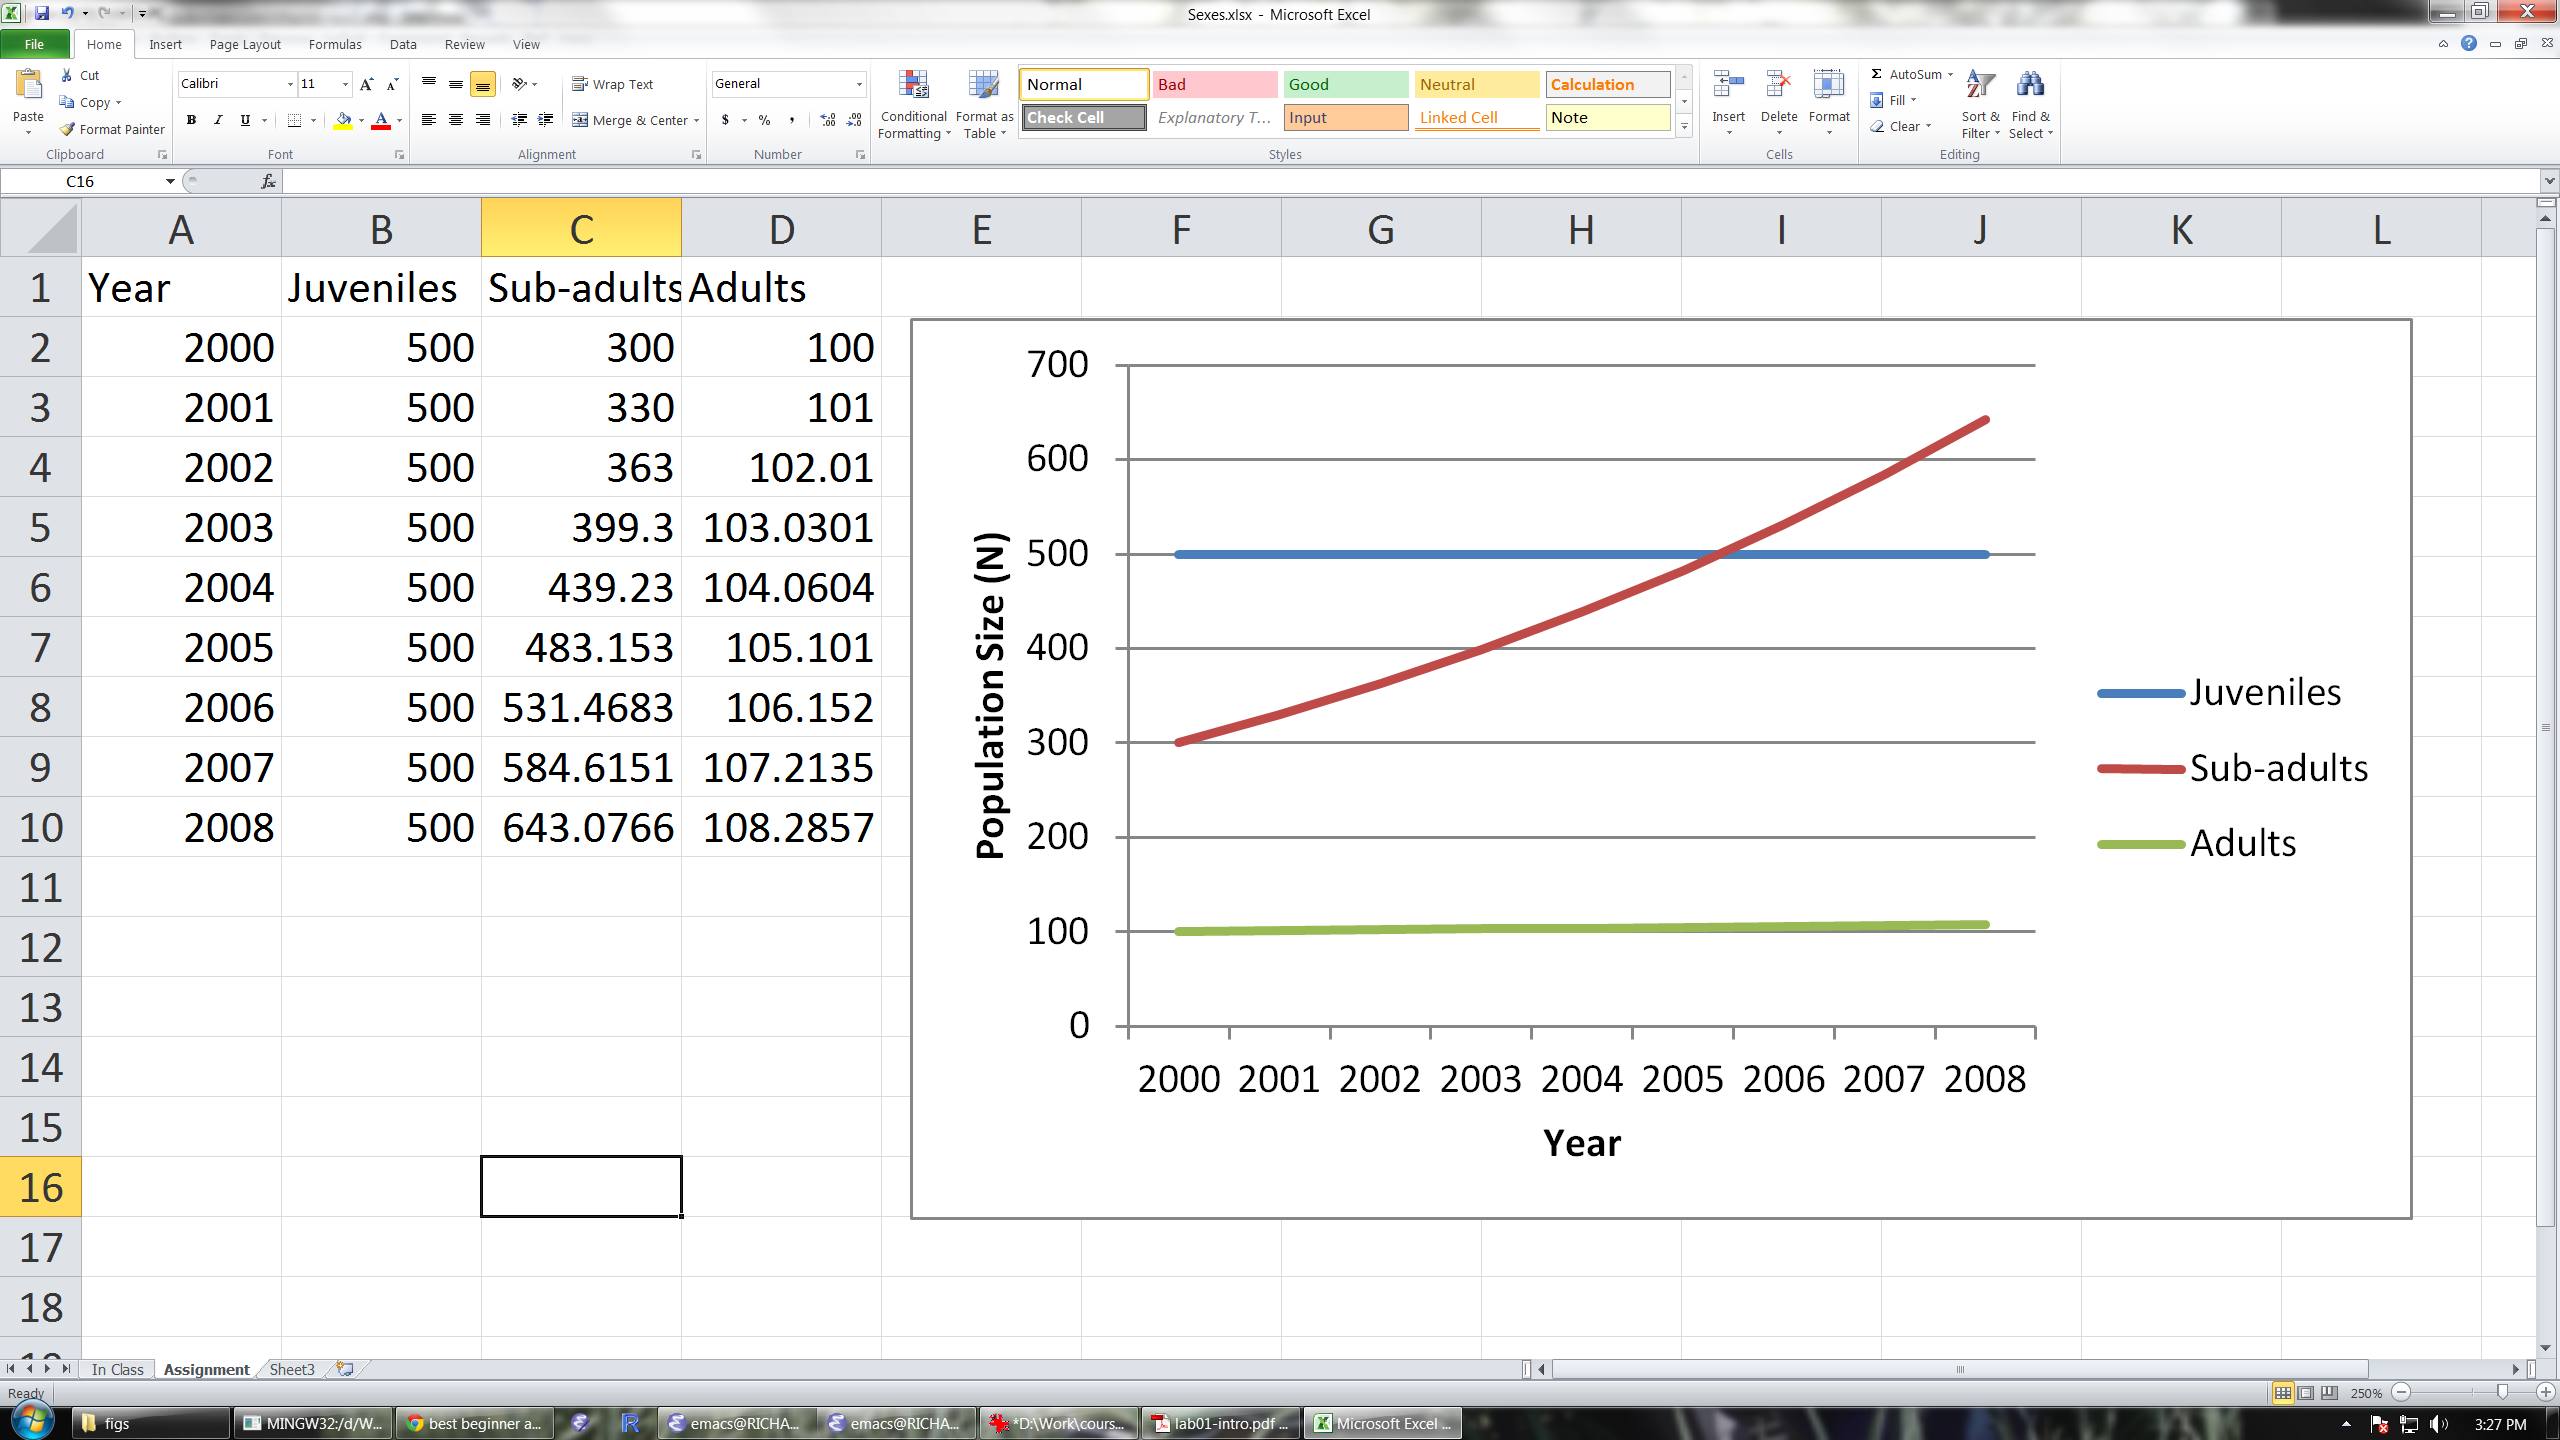
\includegraphics[width=0.7\textwidth]{figs/assignment}}
%   \end{center}
% \end{frame}


\section{R}


\begin{frame}
  \frametitle{R}
  Downloading and installing
\end{frame}


\begin{frame}[fragile]
  \frametitle{Reproducing the Excel exercise}
  Create an object to hold the sequence of years
\begin{knitrout}
\definecolor{shadecolor}{rgb}{0.969, 0.969, 0.969}\color{fgcolor}\begin{kframe}
\begin{alltt}
\hlstd{year} \hlkwb{<-} \hlnum{1950}\hlopt{:}\hlnum{1961} \hlcom{# A vector containing the sequence of years}
\hlstd{year}              \hlcom{# Type the name of an object to see it's values}
\end{alltt}
\begin{verbatim}
##  [1] 1950 1951 1952 1953 1954 1955 1956 1957 1958 1959 1960 1961
\end{verbatim}
\end{kframe}
\end{knitrout}
\pause
\vfill
\begin{knitrout}
\definecolor{shadecolor}{rgb}{0.969, 0.969, 0.969}\color{fgcolor}\begin{kframe}
\begin{alltt}
\hlstd{nYears} \hlkwb{<-} \hlkwd{length}\hlstd{(year)} \hlcom{# Returns the number of values in a vector}
\hlstd{nYears}
\end{alltt}
\begin{verbatim}
## [1] 12
\end{verbatim}
\end{kframe}
\end{knitrout}
\end{frame}


\begin{frame}[fragile]
  \frametitle{A simple population model}
  Create an empty vector to store the data on females
\begin{knitrout}
\definecolor{shadecolor}{rgb}{0.969, 0.969, 0.969}\color{fgcolor}\begin{kframe}
\begin{alltt}
\hlstd{females} \hlkwb{<-} \hlkwd{rep}\hlstd{(}\hlnum{NA}\hlstd{, nYears)}
\hlstd{females[}\hlnum{1}\hlstd{]} \hlkwb{<-} \hlnum{100}
\end{alltt}
\end{kframe}
\end{knitrout}
\pause
\vfill
\begin{knitrout}
\definecolor{shadecolor}{rgb}{0.969, 0.969, 0.969}\color{fgcolor}\begin{kframe}
\begin{alltt}
\hlkwa{for}\hlstd{(t} \hlkwa{in} \hlnum{2}\hlopt{:}\hlstd{nYears) \{}
    \hlstd{females[t]} \hlkwb{<-} \hlstd{females[t}\hlopt{-}\hlnum{1}\hlstd{]} \hlopt{+} \hlstd{females[t}\hlopt{-}\hlnum{1}\hlstd{]}\hlopt{*}\hlnum{0.01}
\hlstd{\}}
\end{alltt}
\end{kframe}
\end{knitrout}
\end{frame}


\begin{frame}[fragile]
  \frametitle{A simple population model}
\begin{knitrout}
\definecolor{shadecolor}{rgb}{0.969, 0.969, 0.969}\color{fgcolor}\begin{kframe}
\begin{alltt}
\hlstd{males} \hlkwb{<-} \hlstd{females}\hlopt{*}\hlnum{0.8}
\hlstd{males}
\end{alltt}
\begin{verbatim}
##  [1] 80.00000 80.80000 81.60800 82.42408 83.24832 84.08080 84.92161
##  [8] 85.77083 86.62854 87.49482 88.36977 89.25347
\end{verbatim}
\end{kframe}
\end{knitrout}
\end{frame}



\end{document}
